%!TEX root = ../thesis.tex

\graphicspath{{Chapter5/Figures/}{Chapter5/Tables/}{Chapter5/Charts/}}

\chapter{The Impact of Team Stability on Structural Metrics}
\section{Introduction} %Section - 5.1 

The previous chapter focused on impact of team size on the structural metrics of software, addressing the first research question (RQ1). In this chapter, the focus turns to the second research question (RQ2):  \textit{the impact of the development team stability on the internal structural metrics of coupling, cohesion, complexity, and modularity of software projects and the implications on its maintainability}. Consistent with the previous chapter, a representative sample is first extracted and a measure of team stability is then presented. This is then used to drive a series of statistical analyses to answer the research question. At the outset of this chapter it is useful to restate the basic definition of team stability as the cumulative time that each team member has worked with their fellow team members. Consistent with the previous chapter, the definition of the team remains the set of unique
committers present in the revision history in the version control system of a given project. This initial basic definition of team stability will be developed and expanded upon through the course of this chapter.

Figure ~\ref{fig:chapter5overview} depicts the structure of this chapter starting with an initial treatment of those aspects of data mining and analysis that are foundational the team stability analysis which is detailed in the latter sections of this chapter. Section 5.2 outlines the approach to conducting network analysis throughout the GoogleCode forge; this is necessary to calculate a reliable measure of team stability. The pitfalls associated with forked projects and multiple committer identities are documented, along with mitigation strategies to these threats to validity. Section 5.3 is concerned with the second strand of foundational work - data mining and preliminary forge analysis to discover those basic trends that have a bearing on the latter analysis phase. Section 5.4 documents the approach to sample extraction necessary for the subsequent analysis in this chapter. Section 5.5 is a study of the impact of \textbf{'intra-project team stability'} on structural metrics; \textit{that is assessing how the stability accrued through the course of the evolution of the project affects its structural metrics, observing the project's final archived state within the forge}. Section 5.6 assesses the impact of \textbf{'inter-project team stability'} on structural metrics; \textit{that is the stability that is gained from retaining committers in a development team across multiple projects}. Inter-project team stability analysis factors in the chronology of projects and makes observations of the impact of stability that accrued in previous projects on structural metrics of the team's subsequent projects. Fortunately, given the breadth of the forge it is feasible to focus exclusively on the study of projects where an entire development team collaborated on a project and subsequently migrated, with the introduction of no new committers, to a later project. A comparison is carried out between the structural metrics of the chronologically earlier project against the later projects and, as in the previous chapter, functional complexity is isolated to remove any confounding impact it may have on the analysis. As in the previous chapter, section 5.7 presents the results in the context of two individual projects.

Figure ~\ref{fig:MiningAnalysisToolchain} highlights, at a high level, aspects of the toolchain that are of relevance to the team stability analysis - aspects that will be expanded on later in this chapter.

\begin{landscape}
\begin{figure}[htbp!] 
\centering    
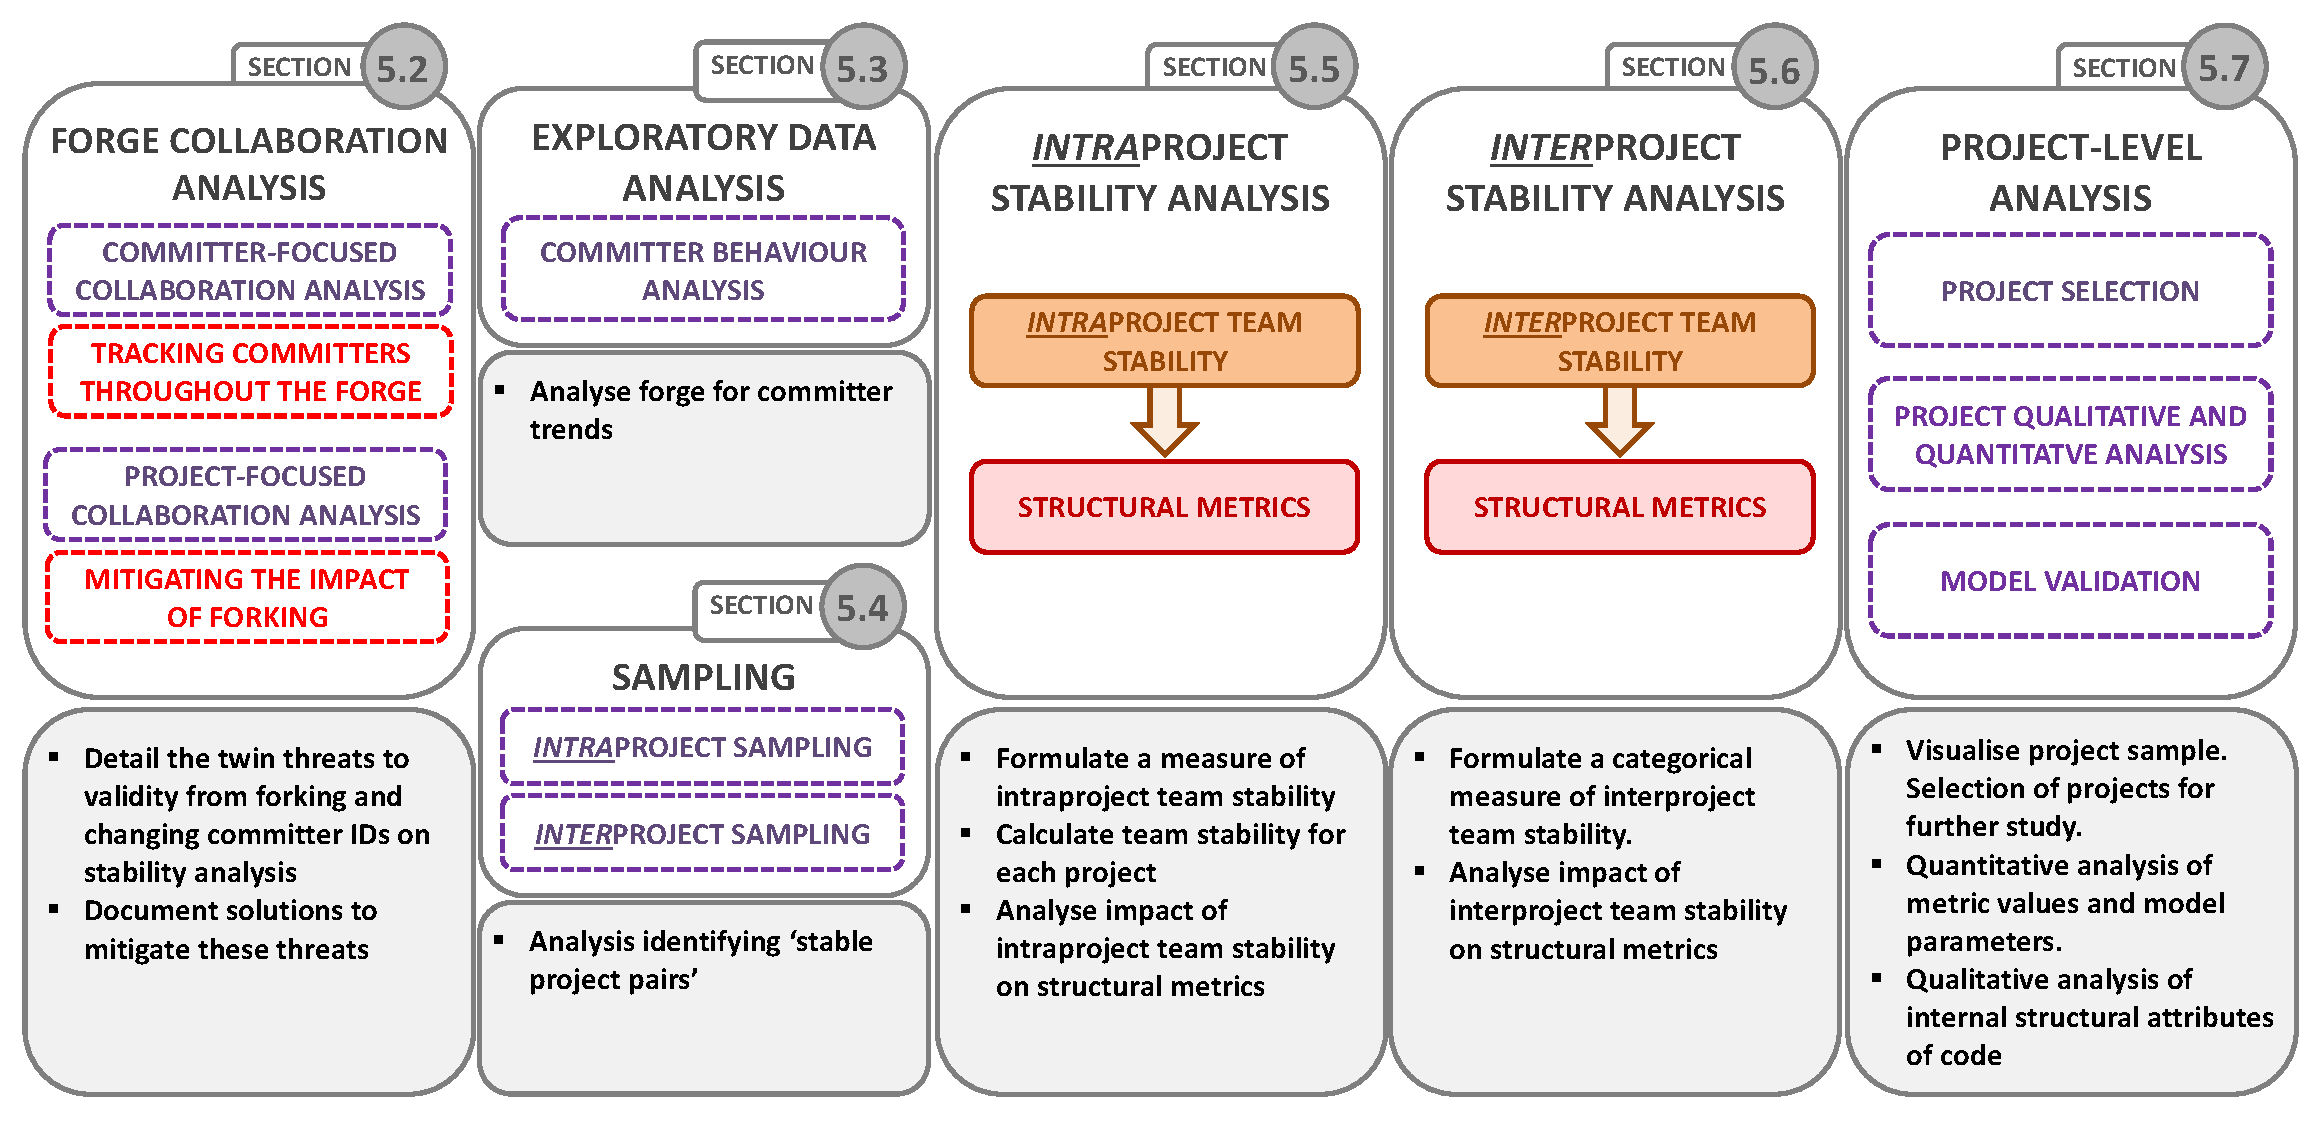
\includegraphics[width=1.3\textwidth]{ChapterOverview.pdf}
\caption{Chapter 5 outline providing an overview of the contents of each section.}
\label{fig:chapter5overview}
\end{figure}
\end{landscape}

\begin{figure}[htbp!] 
\centering    
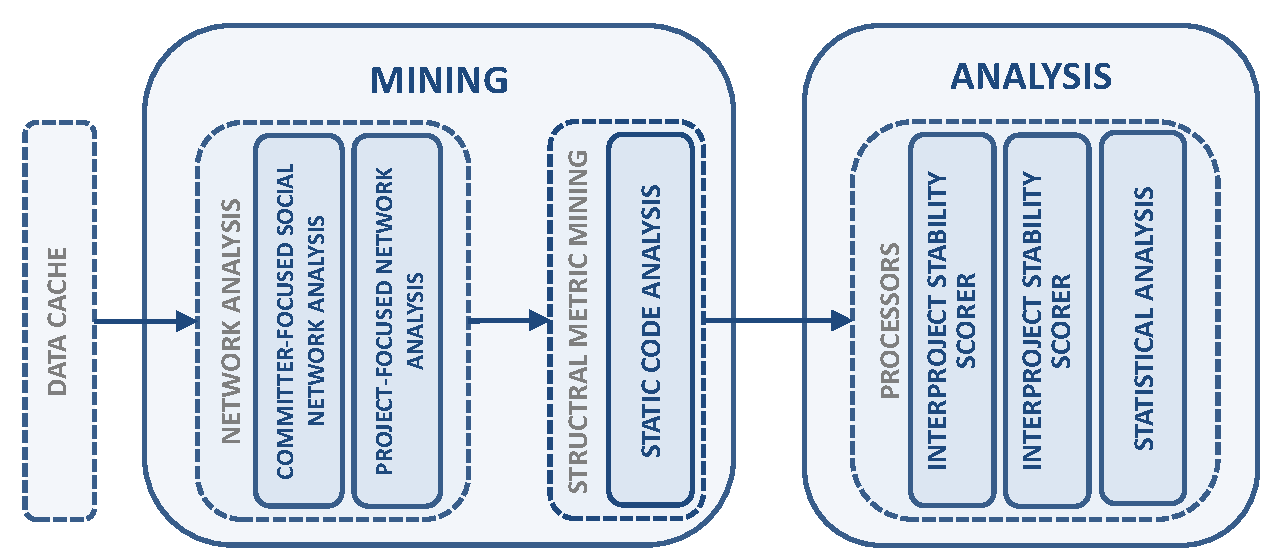
\includegraphics[width=1.0\textwidth]{MiningAnalysisToolchain.pdf}
\caption{Aspects of the toolchain pertinent to team stability analysis.}
\label{fig:MiningAnalysisToolchain}
\end{figure}

\section{Network Analysis} %Section - 5.2 
Network analysis is the process of mapping and measuring relationships between entities. This is a broad subject and there is substantial related work in the field of software development centred on project contributors as the entities to be mapped, usually focussing on studying communication between entities to understand the impact of various organisational dynamics \citep{howison2006social, martinez2008using, conaldi2013dual, daniel2016open, bernardi2018relation}. This research is concerned with utilising network analysis techniques to make accurate observations of team stability that can then be used to drive comparisons between sets of structural metrics.

This research necessitates two types of network analyses illustrated in figure ~\ref{fig:NetworkAnalysis}. The first is a social network analysis focussed on committers where every single commit is mined and mapped to its respective project and the nature of the engagement of each committer's project engagement is analysed within the context of their fellow committers. This is used to calculate the stability of a team through the evolution of the project. 

The second type of network analysis - project-focused network analysis - is concerned with establishing the relationship of projects to one another. This relationship is given rise through the process of 'forking' creating, in essence, a dependency network. As will be discussed in this section, this relationship can distort analysis of committer history hence is it critical that this hierarchy is mapped out in order to eliminate this issue as a potential threat to validity. The project-focused network analysis in this chapter does not consider directionality although this will be discussed in the final chapter as a potential future avenue of work.

This section discusses each of these two types of network analyses separately, their associated mining challenge and the strategy to solve for those challenges.

\begin{figure}[htbp!] 
\centering    
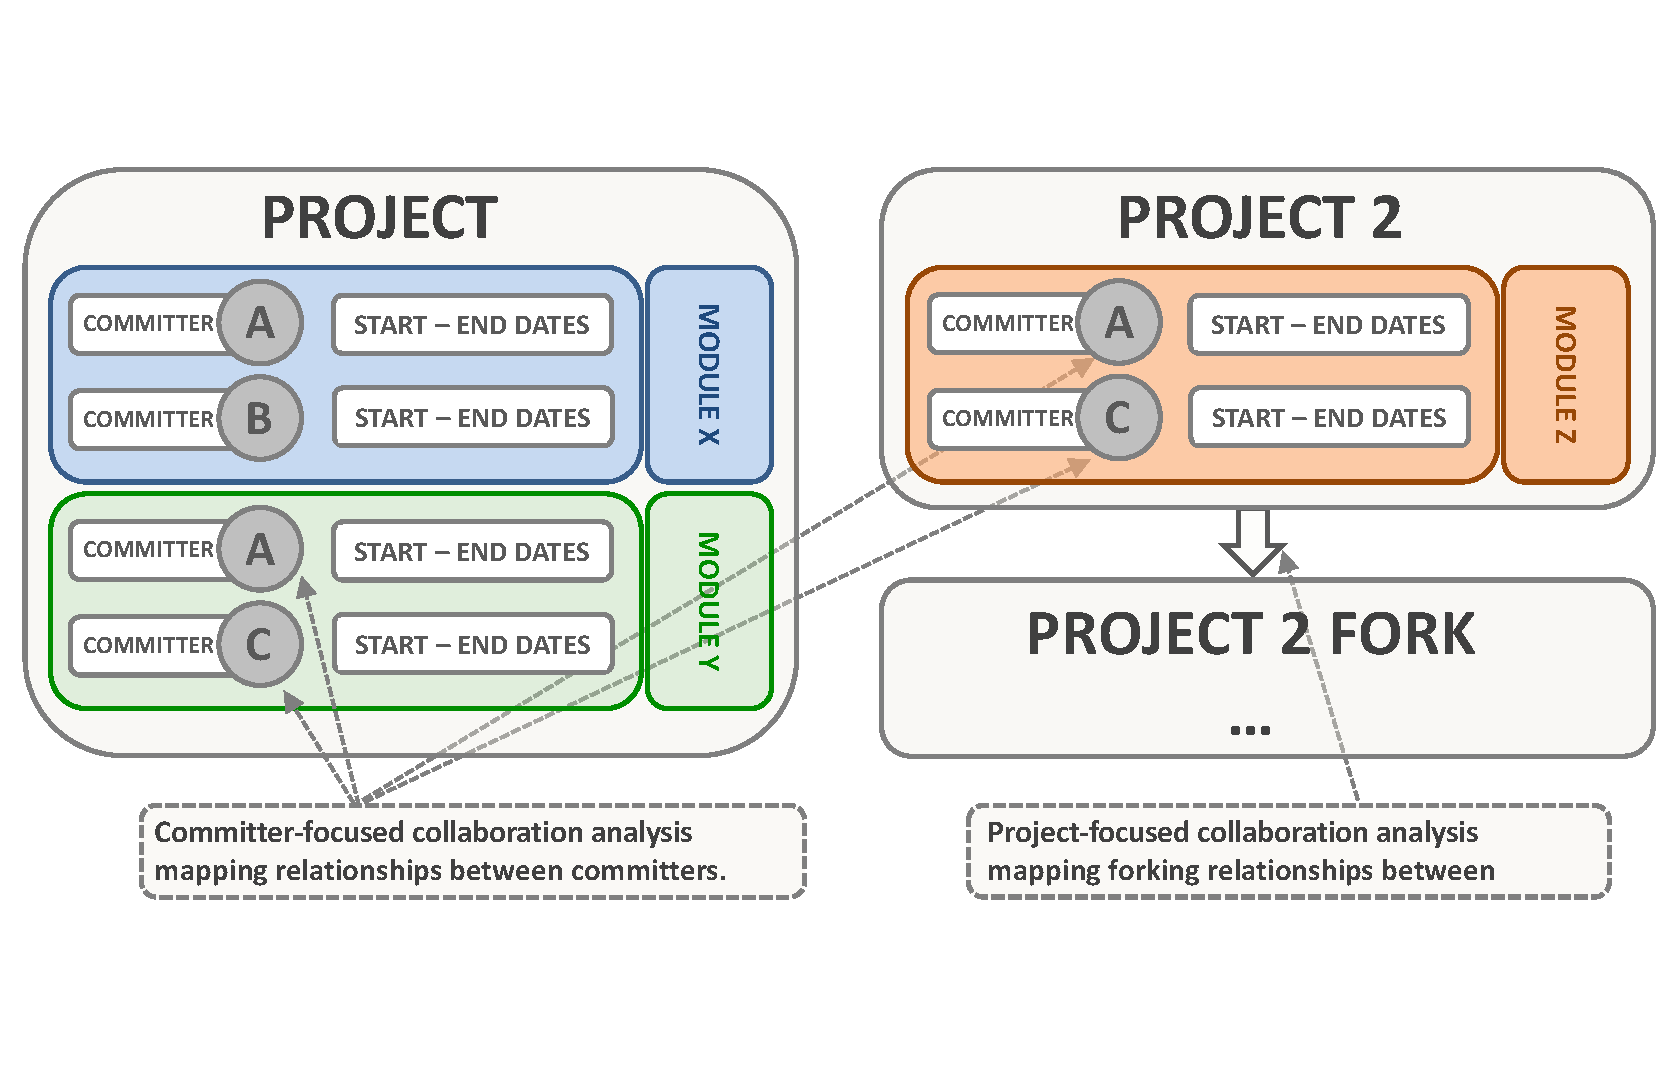
\includegraphics[width=1.0\textwidth]{NetworkAnalysis.pdf}
\caption{A depiction of the network analysis conducted in the GoogleCode forge.}
\label{fig:NetworkAnalysis}
\end{figure}

\subsection{Committer-Focused Social Network Analysis}
The social network analysis strand of this research is concerned with mining the commit history of every committer in the forge, identifying which projects they contribute to, capturing the detail of their project engagement and analysing each committer's project engagement within the context of their fellow committers on those projects. The project engagement detail captured comprises the sub-modules that committers contribute to and the time interval of their contributions. This analysis will provide a basis for the calculation of intra-project team stability to be discussed in more detail in section 5.4.

A challenge to this network analysis is building the capability to consistently track committers as they traverse through the forge. When determining contributor activity, it is noted that multiple user identifiers are occasionally used by the same committer. Without rationalising these to a single identifier it is not possible to effectively track a committer's behaviour. As this research seeks to accurately establish the composition of development teams across all the projects in the forge in order to establish instances where groups of two or more committers contribute to more than one project together, it is essential to reliably identify committers across multiple projects. This is a common problem in the field of mining software repositories and has seen some earlier research efforts. Robles and Gonzalez-Barahona developed a methodology and general heuristics to identify developers across repositories (using data from VCS, mailing lists, and bug reports) \citep{robles2005developer}. They classify email addresses as a 'primary identity' which is almost always present across diverse repositories and they present a general approach to extract identities from email addresses. Applying this approach on the GoogleCode forge, it is observed that multiple email addresses can be attributed to the same identity.

To illustrate by way of example consider the two IDs below which, for the sake of this example, appear in the same project:

\textbf{ID1:} Jane Doe <jane.doe@doe.com> \\
\textbf{ID2:} Jane Doe <jdoe@doe.com>

Robles and Gonzalez-Barahona argue that it is a reasonable assumption that both these user handles refer to the same committer, albeit from two separate user accounts \citep{robles2005developer}. If this is not accounted for in the team stability analysis later in this chapter, this could result in an incorrect determination of the degree of stability attributed to a project.

Fortunately multiple user IDs for a single contributor usually carry sufficient similarity to allow automatic detection and rationalisation of these user IDs. Bird et al. propose a heuristic to rationalise user IDs when mining email social networks \citep{bird2006mining} which is partially adapted and adopted for this purpose. Specifically, there are several stages of name parsing that are applied:

\begin{itemize}
\item Where a name is accompanied by an email address in brackets the email address is ignored. In this case one user ID would be selected to which we assign the commits of both user IDs.
\item All names are converted to lower case and all trailing spaces are removed.
\item All punctuation is removed and replaced with a single space.
\item Multiple spaces are replaced with a single space.
\end{itemize}
 
When this type of network analysis is applied to the GoogleCode forge, it is observed that 17\% of unique committer identities are indeed sufficiently similar to be considered subtly different identities referring to the same committer. Naturally, activities on these alternate identities are conflated to represent a comprehensive view of the committer's behaviour.
 
\begin{figure}[htbp!] 
\centering    
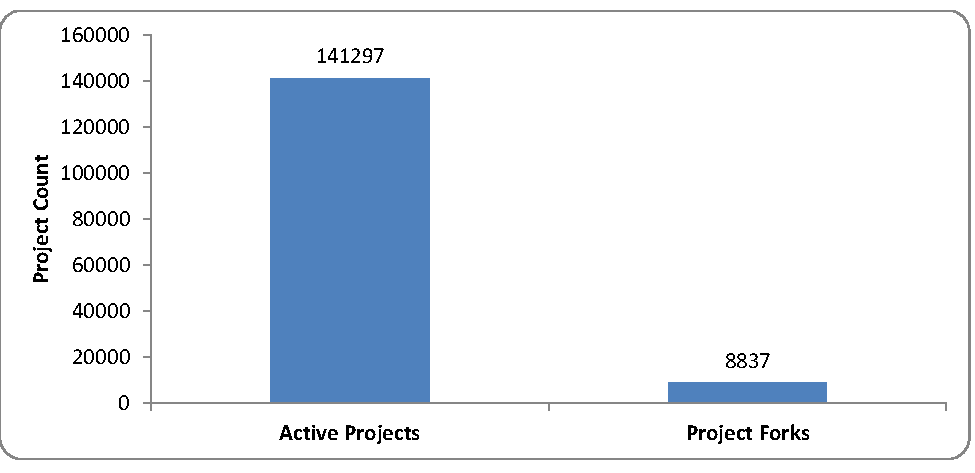
\includegraphics[width=1.0\textwidth]{ForkCounts.pdf}
\caption{A depiction of the number of committers in the GoogleCode forge pre- and post-analysis.}
\label{fig:ProjectCommitterPrePostCleanup}
\end{figure}

\subsection{Project-Focused Network Analysis}
The project-focused network analysis within this research is concerned with mapping out the parent-fork relationships between projects. Forking refers to the process of creating an alternate and independent software development stream from an existing project. When unmapped, these relationships can pose a real threat to validity due to the duplication of commit history in the child project which can erroneously reflect those committers contributing to the parent project also contributing to the child project. This research seeks to study inter-project stability by studying projects where groups of committers genuinely contributed to multiple projects. Therefore this type of network analysis is necessary to avoid misattributing duplicated commits from forked projects to committers who have not genuinely contributed to those projects. 

\newline
\textbf{5.2.2.1 Mechanics of Forking}
\newline
One of the strengths of open-source software development is the ease with which one can start a new project leveraging all the tools that an open-source forge can offer. An unsuccessful project will attract few additional contributors while a successful project will build an active development community, produce artefacts and ultimately an active user base. Open-source forges also simplify the process of starting new projects based on the source code of existing projects and without affecting the original. The motivations to do so can range from discontent at the direction of development in the 'master' project through to a desire to build or experiment with new ideas within a mature project. The process of forking is named as such after the concept of forking processes to execute in parallel.

Forking projects can take multiple forms and each presents its own challenges in terms of automated detection. For the avoidance of doubt, when 'forking projects' are referred to, this is distinct to the 'fork and pull' development approach adopted by repositories such as GitHub, studied extensively by Kalliamvakou et al. \citep{kalliamvakou2014promises}. 'Fork and pull' is the process of cloning a master repository into an individual contributor's personal repository which acts as a staging area before changes, after review, can be merged into the master repository. This research, however, is concerned with forked projects that represent an entirely different development stream to the original project.

The process of creating a fork of a project can take several forms. This section discusses each approach illustrating using examples from GoogleCode.

\begin{itemize}
\item \textbf{Copying source files or binaries}
Some developers choose to fork projects by copying selected elements of the parent project's codebase. This could, for example, take the form of copying selected pre-compiled binaries or indeed the entirety of the source code. The example depicted in Figure ~\ref{fig:ForkedImportedBinaries} illustrates a snapshot of the revision history of the 'iTerm2' project - a MacOS Terminal replacement - which is a fork of the iTerm project. The second of the two revisions (r2) shows an import of the source files of the parent project. At the heart of this threat is that there is essentially no way of determining if a committer's contribution is their original work or whether it was fully or partially copied from other projects or sources without mining a host of other forges. While this is not a serious threat to the validity of this research, this could impact those researchers attempting to understand the value of developer contributions and would necessitate a mechanism to distinguish between a committer's original source code and that imported from other projects. For this reason, among others, development of techniques and software to identify 'code cloning' is an active field of research \citep{roy2009comparison}. While Brixtel et al. presented a framework which could be deployed for the purposes plagiarism detection \citep{brixtel2010language}, the majority of the efforts in this field focus on gaining greater understanding on the evolution of software repositories and reducing the wasted effort arising from duplicate code. Juergens et al. created an open-source workbench for code detection research geared towards configurability and extensibility and hence designed to support code clone research \citep{juergens2009clonedetective}. Lee et al. worked designed algorithms to support scalable indexing structures on vector abstractions of code to allow for the rapid detection of clones \citep{lee2010instant}. This work will be discussed towards the latter part of this thesis in the context of possible future work.

\begin{figure}[htbp!] 
\centering    
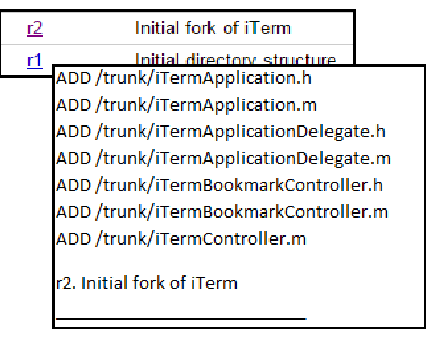
\includegraphics{ForkedImportedBinaries.pdf}
\caption{A snapshot of the start of the commit history of the 'iTerm2' project.}
\label{fig:ForkedImportedBinaries}
\end{figure}

\item \textbf{Cloning a repository within the forge}
Most popular version control systems make it fairly easy to clone a project, along with its full commit history into a new repository. Where this approach is taken to create a new fork, it will have an identical history to its parent. Figure ~\ref{fig:ForkedSameHistory}  shows the identical VCS history of the 'hotcakes' and 'zumastor' projects - both enterprise network storage solutions. In this example both projects share the same first 239 commits, after which they take divergent development paths. When conducting network analysis across the forge, without factoring in this threat to validity, it may be falsely observed that the committers of 'hotcakes' later contributed on 'zumastor'.

\begin{figure}[htbp!] 
\centering    
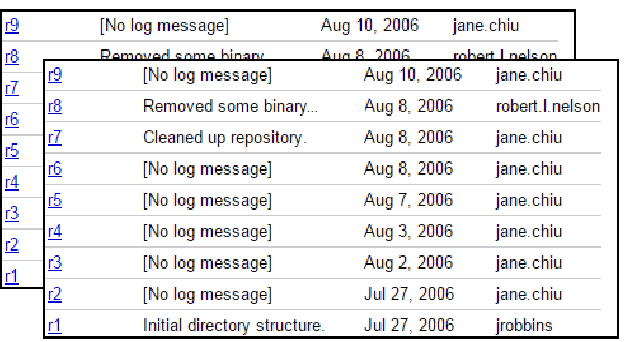
\includegraphics{ForkedSameHistory.pdf}
\caption{The identical VCS history of the 'hotcakes' and 'zumastor' projects.}
\label{fig:ForkedSameHistory}
\end{figure}

\item \textbf{Cloning a repository from outside forges}
This approach is a subtle variation on the previous method. Figure ~\ref{fig:ForkedOutsideForge} depicts the commit history of the 'cacheboy' project repository - a fork of 'squid' which is a webserver caching solution. Commits predate GoogleCode's launch by 9 years so clearly cannot be part of the 'cacheboy' project itself. These commits do, in-fact, belong to the 'squid' project which was hosted on a repository external to the GoogleCode forge. The existence of a parent outside the open-source forge will prove a challenge to detect. The threat to the validity of the network analysis in this case is the erroneous attribution of committer activity to a fork rather than a parent that resides outside the forge. This threat is of no consequence to this research given that the parent resides outside GoogleCode, there is no threat of 'double counting' the committer contribution; the risk is solely that the aggregate activity across the two projects is assigned to the later forked project. 
 
\begin{figure}[htbp!] 
\centering    
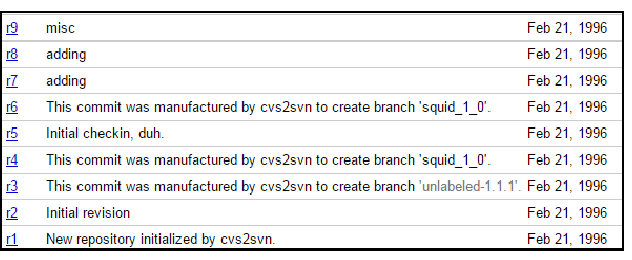
\includegraphics{ForkedOutsideForge.pdf}
\caption{The VCS history of CacheBoy.}
\label{fig:ForkedOutsideForge}
\end{figure}

\end{itemize}

\newline
\textbf{5.2.2.2 Identifying Forked Projects}
\newline
Identifying forked projects is an area which has seen some prior academic interest. Nyman and Mikkonen conducted research to establish the most common motivations for forking within SourceForge \citep{nyman2011fork}. The methodology to identify forked projects was to search the project descriptions that referred to forking. Although this approach suffices when attempting to locate a sample to study, relying on developers to specifically declare a project as 'forked' in the description does not help us identify a comprehensive set of forked projects to facilitate an accurate network analysis. Similarly, Robles et al. \citep{robles2012comprehensive} used a fairly manual approach for locating significant software forks that involved searching Wikipedia using the term 'software fork' and manually navigating to the project homepage to extract key information ahead of a study on the motivations and outcomes of forking. Again this cannot be applied to the large-scale mining of software forks within open-source forges making this approach inappropriate to identifying a comprehensive set of forks. 

As part of the process of maintaining a forked project, it is often desirable or indeed necessary to import changes from the master project. Ray and Kim developed a tool called REPERTOIRE to automate the identification of commonality between known forked projects through comparison of source files but it does not attempt identify forked projects in a wider open-source forge \citep{ray2012repertoire}. Of the approaches to automated clone detection, this is closest to the methodology adopted in this research. While REPERTOIRE tracks activity between known forked projects, this research is focussed on identifying the forked projects the co-exist within a forge. As such, this research can be considered complementary to the work of Ray and Kim.

This research proposes a heuristic which searches for common commits across projects and identifies them as projects exhibiting a fork relationship. Limitations to the heuristic tare outlined below.

\begin{itemize}
\item  \textbf{Coverage:} This approach is only capable of detecting forks where the parent also resides in the forge (or set of forges) being analysed; i.e. the mechanism of forking earlier referred to as 'cloning a repository within the forge'. This is not a limitation within the context of this research as this analysis is concerned with identifying those inter-project relationships that arise as a result of forking projects within the forge. This is because this forking mechanism was earlier identified at the only mechanism that has the capacity to create a distortion to the type of committer-focused network analysis conducted in this research. 
\item  \textbf{Forks by source file import:} As detailed earlier, some projects are forked by importing binaries and source files from other projects rather than importing the version control commits themselves. These forked projects are not detected by this heuristic but may be found by the other heuristics if the project or commit description contains the term �fork�. Again, this is not a limitation in the context of this work as these other forking mechanisms do not pose a threat to the validity of the network analysis in the latter parts of this chapter.
\item  \textbf{Context limitations:} This heuristic does not attempt to establish which, within a forking relationship, which project is the parent and which is the child. While establishing this relationship can be informative, as will be outlined in the Discussion chapter, it is not necessary for the purposes of the committer-focused network analysis in this research.
\end{itemize}

Figure ~\ref{fig:ForkCounts} shows the results of this analysis. 6.25\% of projects in the GoogleCode forge are forks of parent projects with a revision history that contains commits that are duplicated from the parent project. 

\begin{figure}[htbp!] 
\centering    
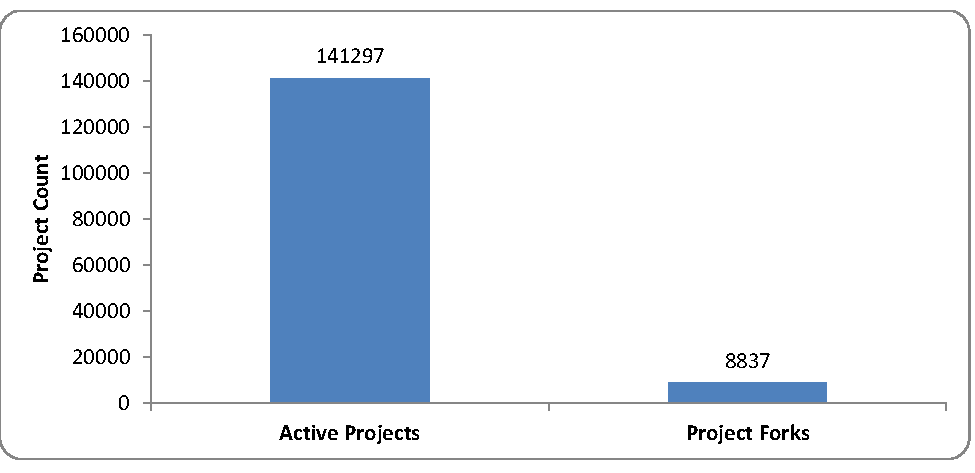
\includegraphics[width=1.0\textwidth]{ForkCounts.pdf}
\caption[A chart comparing the total number of active projects to the number of project forks.]{A chart comparing the total number of active projects (i.e. those projects with commits beyond the initial repository creation commit) to the number of project forks.}
\label{fig:ForkCounts}
\end{figure}

\section{Exploratory Data Analysis} %Section - 5.3
This section studies basic committer behaviour in order to analyse typical project engagement. This basic preliminary analysis will be valuable when conducting network analysis to calculate team stability.

Figure ~\ref{fig:LogCommitterCountProjectsEngaged} depicts the number of distinct projects that individual committers engage in, plotted against the log of the number of committers with that project engagement count. While 87\% of committers engage in a single project only, there are substantial numbers of committers that engage in multiple projects. This is significant as it indicates the availability of multiple committers engaging multiple projects - something that is critical for the identification of the inter-project team stability analysis data set as discussed in the next section.

Figure ~\ref{fig:FrequencyEngagement} is a representation of the duration of committer project engagement. This is calculated as the elapsed time (in units of days) between the first and last commits of individual committer on a project and is plotted against the frequency of that duration across all committer project engagements. It is observed that the majority of project engagements have a duration of eleven days or more. This has implications for the accumulation of intra-project team stability and, again, makes it likely that significant time overlaps between committers within a single project will be observed. As will be discussed later in this chapter, this is necessary for the accumulation of intra-project stability through the evolution of a project.

\begin{figure}[htbp!] 
\centering    
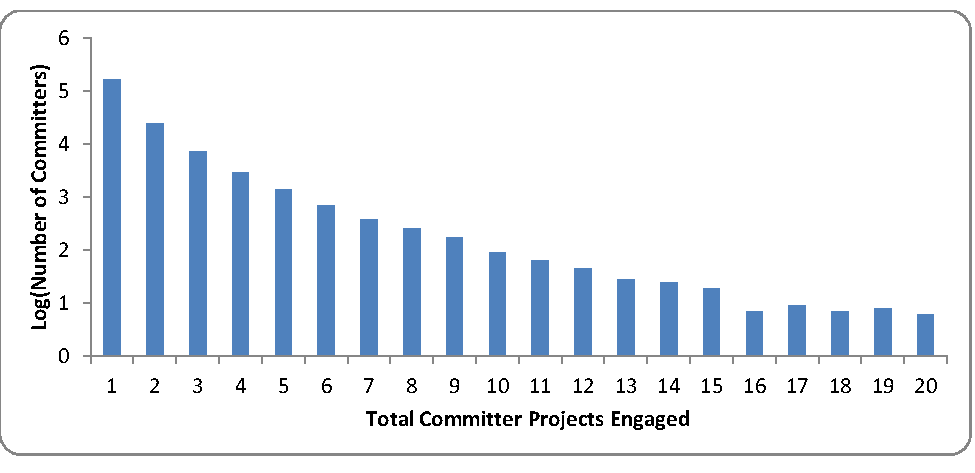
\includegraphics[width=1.0\textwidth]{LogCommitterCountProjectsEngaged.pdf}
\caption{The number of projects individual committers contribute to throughout GoogleCode.}
\label{fig:LogCommitterCountProjectsEngaged}
\end{figure}

\begin{figure}[htbp!] 
\centering    
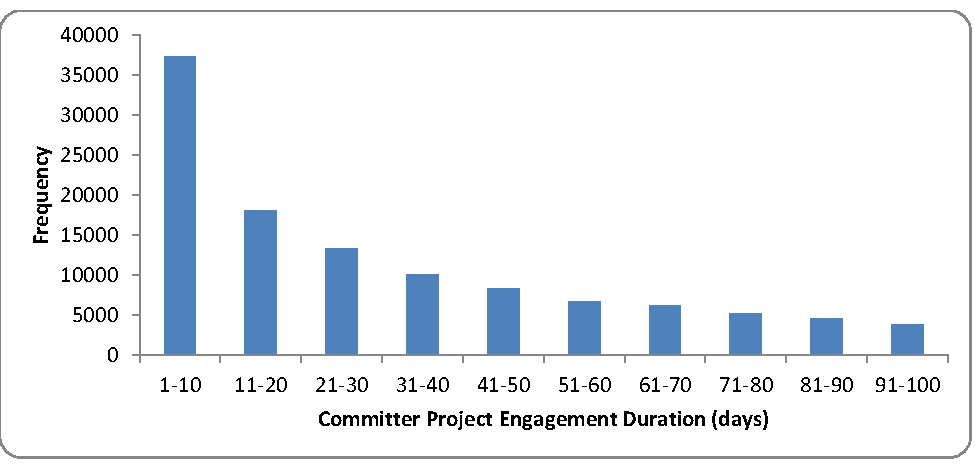
\includegraphics[width=1.0\textwidth]{FrequencyEngagement.pdf}
\caption[The frequency of the timespan of project engagement.]{The frequency of the timespan of project engagement - measured as the time between the first and last commits on projects by individual committers.}
\label{fig:FrequencyEngagement}
\end{figure}


\section{Sampling} %Section - 5.4
The network analyses detailed earlier underpins the team stability analysis which is necessarily based on an accurate and comprehensive picture of committer project contributions and forge traversal. Where \textbf{intra}-project stability is studied, it is necessary to map the individual committer contributions at the project level. This type of analysis places limited demands on the requisite data set. Projects included in the data set should have more than one committer as there can be no meaningful analysis unless there are multiple committers. As with the team size analysis, it is possible to continue to restrict the study to Java projects only without unduly compromising the sample size. 

\textbf{Inter}-project stability analysis places greater demands on the data data-set and essentially should comprise pairs of projects where multiple committers migrate from a project, potentially shedding committers but not gaining any new ones, onto a new project. In order to provide contrast between the later project where committers have established some stability in comparison to the earlier project where the team stability would have been less, there should be no time overlap in the commit activity of the two projects. This criteria is illustrated in figure ~\ref{fig:ProjectPairEligability} below. The earlier project network analysis ensures that we reliably identify these project pairs without the distortion that forking can bring.

The network analysis discussed in section 5.2 enables the accurate and comprehensive mapping of committer project engagement throughout the forge. This facilitates the identification of projects where committers have contributed to more than one project alongside the same fellow contributors. This forms what is termed in this thesis a \textit{'stable partnership'}; i.e. two or more committers contributing to two or more of the same projects. This stable partnership is associated with a 'stable project pair'; this is to say that pair of projects where the 'stable partnership(s)' manifest. This is a simplification as there could be more than two projects where these partnerships appear. For the purposes of ascertaining the impact of stability this does not constitute a threat to validity, rather it is an opportunity for further work as will be discussed in the next chapter.

The expansive nature of the GoogleCode forge enables the application of fairly specific criteria to the identification of the inter-project analysis data set while retaining a statistically significant sample size. As illustrated in figure ~\ref{fig:ProjectPairEligability}, only project pairs where the commit history of the earlier of the projects concludes before the later project commences are included in the data set. This is to ensure that stable partnerships are captured rather than overlapping partnerships which could detract from the impact of the team's stability. Secondly, only those project pairs with committer populations entirely made of stable partnerships are eligible for inclusion; that is to say that the committers in the later project in the pair should be made up entirely of contributors from the earlier project. This is to avoid considering projects where the inter-project team stability is reduced by newcomers to the team. Finally, as discussed earlier in this chapter, the population sample must be cleansed of  forked projects with duplicated commit history as this is essentially distorted information which would constitute a threat to validity. 

\begin{figure}[htbp!] 
\centering    
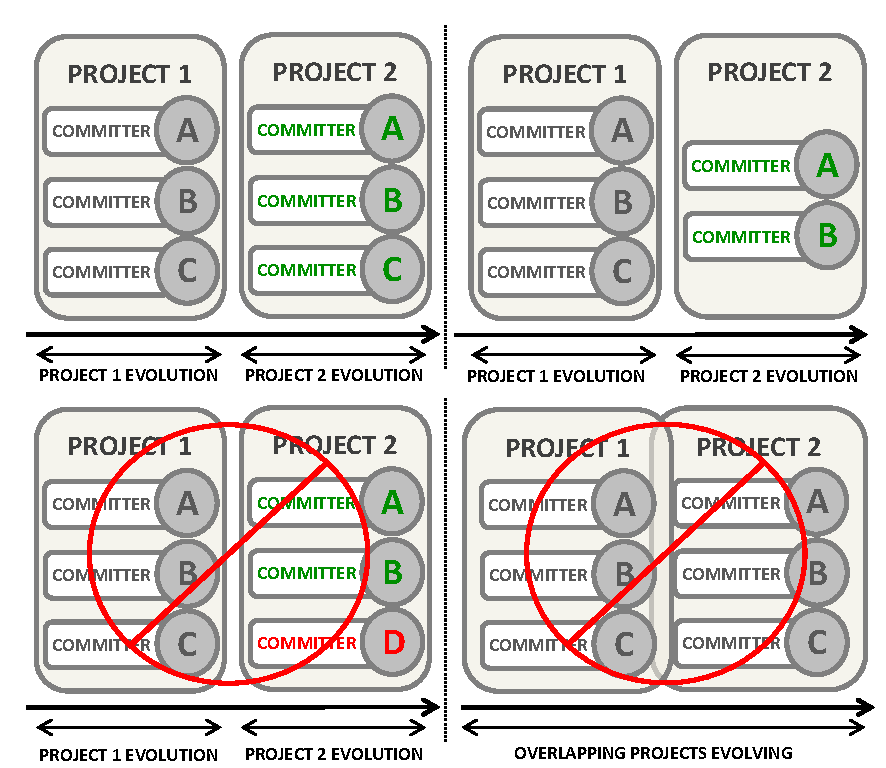
\includegraphics[width=1.0\textwidth]{ProjectPairEligability.pdf}
\caption[An illustration of the 'project pairs' that are eligible for inclusion in the intra-project stability analysis.]{An illustration of the 'project pairs' that are eligible for inclusion in the intra-project stability analysis. While shedding team members from one project to the next is acceptable, additional committers is not. Projects must not overlap.}
\label{fig:ProjectPairEligability}
\end{figure}

This comprehensive criteria enables the creation of two distinct data-sets which can then be analysed relative to one another; projects where committers have previously partnered together 0 to \textit{n} times against those later projects where they have partnered 1 to \textit{n+1} times. By contrasting the structural metrics of each of the earlier projects within a stable project pair against the later project within that pair, it is possible to make some observations on the impact of team stability on these structural attributes of these projects.

For simplicity, once the data set for the inter-project stability analysis is identified, that same data set is leveraged to drive the intra-project stability analysis where projects are studied in isolation as opposed to within a their project pair.

The execution of this network analysis yields 411 project pairs - 822 projects in total. Figure ~\ref{fig:ProjectCommitterCount} shows the committer counts across the sample, with the vast majority of projects exhibiting single digit committer counts. This trend is consistent with the observed trends in the forge analysis in the prior chapter as illustrated in figure ~\ref{fig:CumulativeCommitterCount}.

\begin{figure}[htbp!] 
\centering    
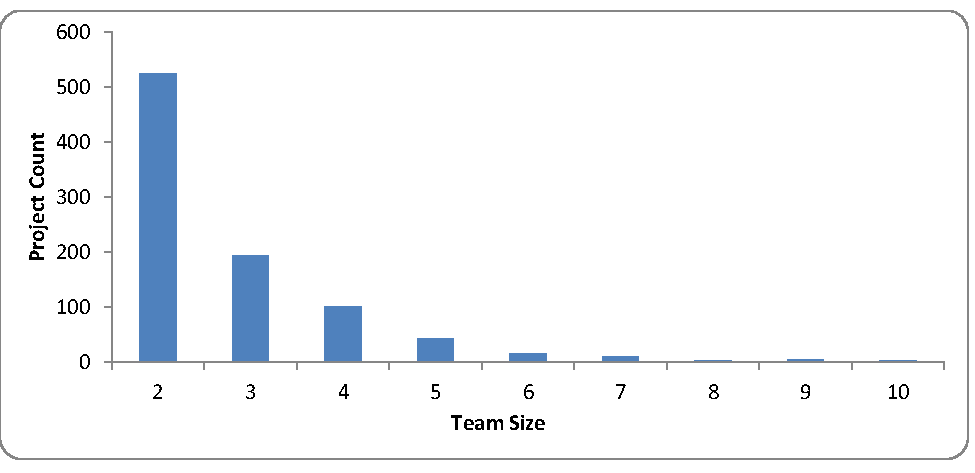
\includegraphics[width=1.0\textwidth]{ProjectCommitterCount.pdf}
\caption{Committer counts across the sample, with the vast majority of projects exhibiting single digit committer counts.}
\label{fig:ProjectCommitterCount}
\end{figure}

\section{Intra-project stability analysis} %Section - 5.4
The earlier definition of team stability - the cumulative time that each team member works with their fellow team members - is fairly broad and open to interpretation. This section provides greater precision around this definition and proposes a calculation for intra-project team stability - a measure capturing the degree of stability accrued by a team through the course of a project. 

\subsection{Determining a measure of intra-project stability}
This research proposes a measure of stability, assigned at a project-level, to capture the degree to which committers on a project accrue time working alongside their peers on the project. The premise of this measure relates to the earlier definition of stability from Huckman et al. which states that the greater cumulative time that a team of committers spend working with each other, the more stable that team \citep{huckman2009team}. 

Before delving into the specifics of how this measure is calculated, it is helpful to first explain that, within this model, there are two main constructs. The first is the 'time-frame of activity'. This applies both at level of the committer and the project and is defined as the window of time stretching from the first and last commits for that entity; specifically only those commits that impact Java source code, excluding for example, documentation changes. For instance, if a project records its first commit on the first day of January and its final commit on the final day of December of that same year, it would have a time-frame of activity spanning the 365 days of that year. Likewise, a committer recording commits on the first and last day of January would have a time-frame of activity spanning the 31 days of that month.

\begin{figure}[htbp!]
\centering
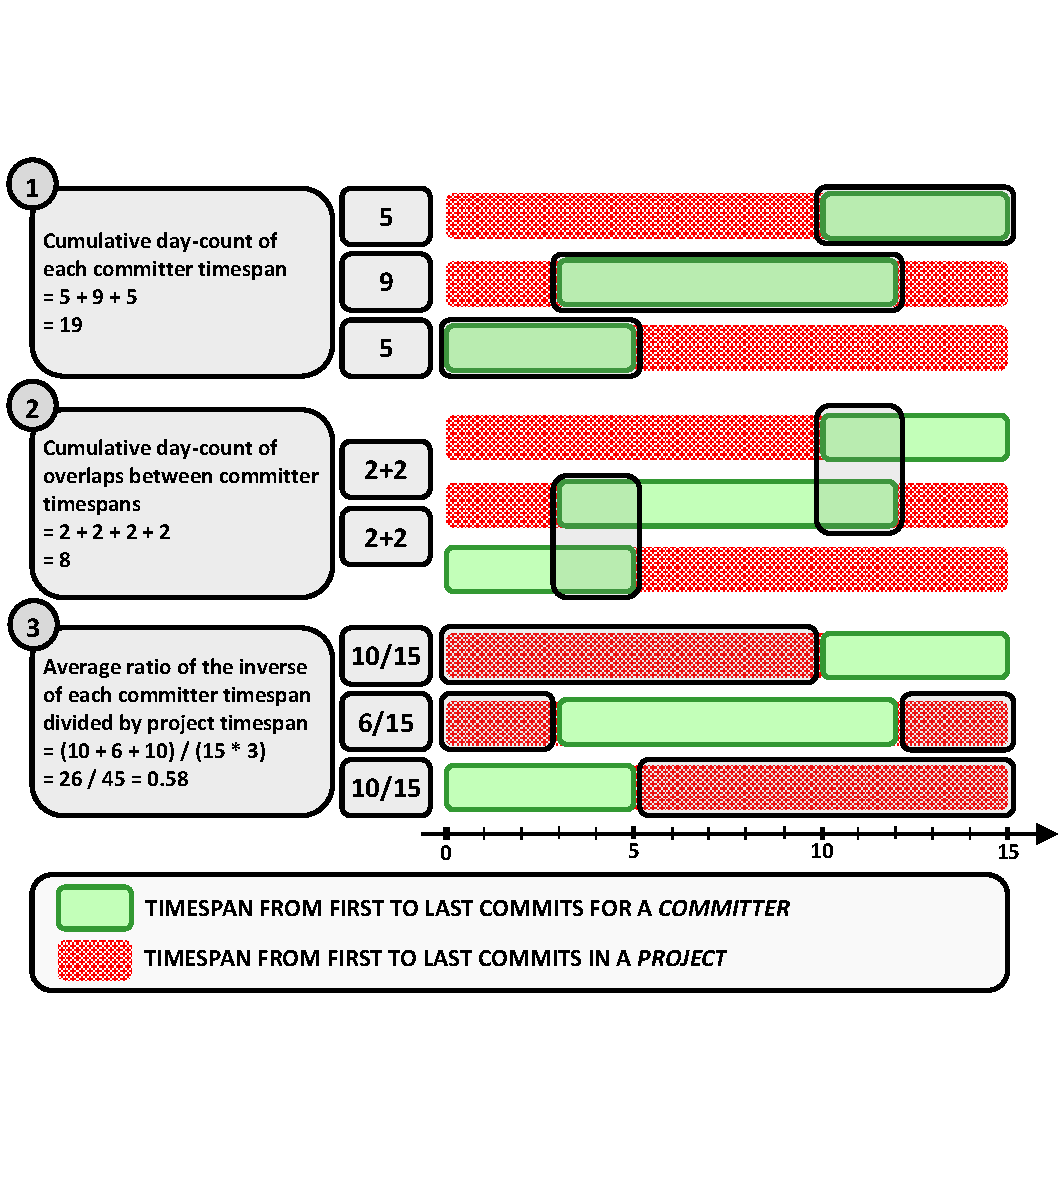
\includegraphics[width=1.0\textwidth]{IntraprojectStabilityCalcOptions.pdf}
\caption{A hypothetical example showing three different approaches to calculating intra-project stability.}
\label{fig:IntraprojectStabilityCalcOptions}
\end{figure}

The second construct relates to how stability (or lack thereof) accrues on a project. Figure ~\ref{fig:IntraprojectStabilityCalcOptions} outlines three mechanisms through which a measure of stability can be derived. The first method (labelled '1') is the most straightforward and is to directly capture the number of days in each committers time-frame of activity through the course of the project. This is the most simplest transposition of the Huckman definition onto this problem space. However, it is also a measure that will closely track team size and does not capture the degree to which time-frames of activity overlap. The second method does capture the cumulative number of days that that these time-frames of activity overlap but will also be closely correlated with team size. The third method captures the extent to which the committer time-frames of activity \textit{do not align} with that of the project's time-frame of activity and therefore often misaligning with their peers and failing to accrue stability. For the reasons outlined below, this third method is chosen for this work and the measure is termed the 'Lack of Stability Ratio (LSR).

\begin{itemize}
\item  \textbf{Avoiding tracking team size:} As illustrated in Figure ~\ref{fig:IntraprojectStabilityCalcOptions}, the first two methods risk primarily tracking team size rather than stability. LSR, however, calculates a ratio which captures a particular aspect of committer time-frames of activity and therefore avoids tracking team size.
\item  \textbf{Adhere to conventions:} By measuring 'lack of stability' rather than 'stability', LSR continues the convention set by the CK metric suite and other software metric suites that favourable measures are lower in value (Lack of Cohesion being a pertinent example).
\end{itemize}

\subsection{Calculating LSR in practice}
An example of how LSR is calculated on a project from the stability project sample is illustrated in Figure ~\ref{fig:IntraprojectStabilityCalc}. The LSR calculation is based on the Jaccard Index where similarity is established between each and every committer time-frame of activity to the overall project time-frame of activity. 

The Jaccard index is the simplest of several similarity measures and was developed at the start of the previous century to compare botanical data sets \citep{jaccard1901distribution}. The Jaccard Index has some prior use in the field of mining software repositories. Kiefer et al. and Kpodjedo et al. use this measure to calculate similarity between Java classes to observe evolution of software projects through releases \citep{kiefer2007mining, kpodjedo2013studying}.  Jermakovics et al. used the measure to compute similarities among developers based on common file changes, constructing a network of collaborating developers \citep{jermakovics2011mining}.   Alternative similarity measures such as the S{\o}rensen-Dice coefficient \citep{sorensen1948method} or Euclidean distance add complexity but it isn't clear that either would better capture team stability given that they are more suited to weighting certain factors and clustering respectively. The Jaccard Index is defined as the size of the intersection divided by the size of the union of the sample sets.		

\newline
\[J(A,B)\ = \frac{\left |A\bigcap B \right |}{\left |A\bigcup   B\right |}\]

While the Jaccard Index is designed to establish the similarity between two finite data sets, the LSR calculation is an adaptation of this approach to take into account the fact that there can be more than two committer time-frames that need to be factored into the stability ratio. It is essential that LSR is in the form of a ratio to avoid calculating a number which has a strong direct correlation to committer count which would simply lead to tracking that factor and, ultimately, confounding results. As expressed in the equation below, LSR is the inverse of the simple means of the Jaccard Indexes of each unique pair of committer time-series:

\newline
\newline
\[\large LSR \ = 1 - \frac{ \frac{Committer \mathit{1} \ \bigcap\ Committer\ \mathit{2}} {Committer\ \mathit{1}\ \bigcup\ Committer\ \mathit{2}} \ ...\ n } {n}\]

\begin{figure}[htbp!]
\centering
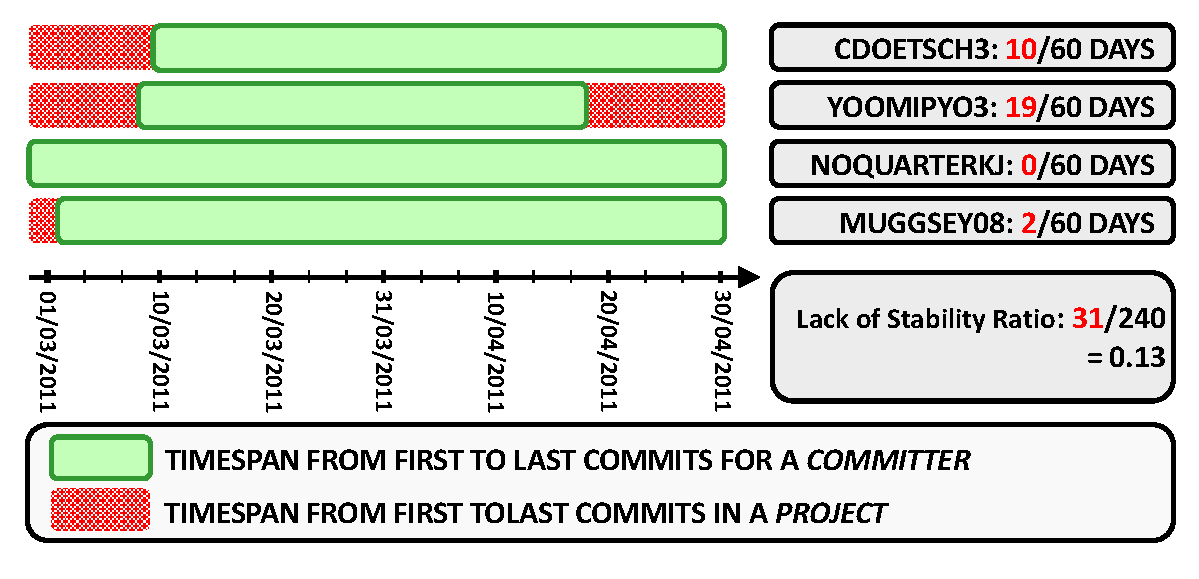
\includegraphics[width=1.0\textwidth]{IntraprojectStabilityCalc.pdf}
\caption{A worked example showing the calculation of the Lack of Stability Ratio (LSR) in a project called 'TeamAwesomeExpress' from the stability project sample.}
\label{fig:IntraprojectStabilityCalc}
\end{figure}

While the previous example is valid, it is also true that many software projects - particularly larger ones - are commonly divided into 'modules'; a fact that should be factored in the calculations. Each module represents a logical grouping of functionality with its source code typically residing in its own folder within the project repository. The concept of modules helps decouple sections of the codebase, providing the ability for specialisation amongst team members and reducing the need for coordination between them. Where the definition of team stability refers to team members 'working together', this should be expanded to stipulate that they work together on the same module, as otherwise there can be no assumptions on the degree of coordination between members - coordination being crucial to the accruing of stability in a team. 

Figure ~\ref{fig:ProjectModuleCount} shows the prevalence of multi-module projects throughout the stability analysis data set. Figure ~\ref{fig:IntraprojectStabilityCalcModularised} illustrates a worked example of a stability ratio calculation of a multi-module project.

\begin{figure}[htbp!] 
\centering    
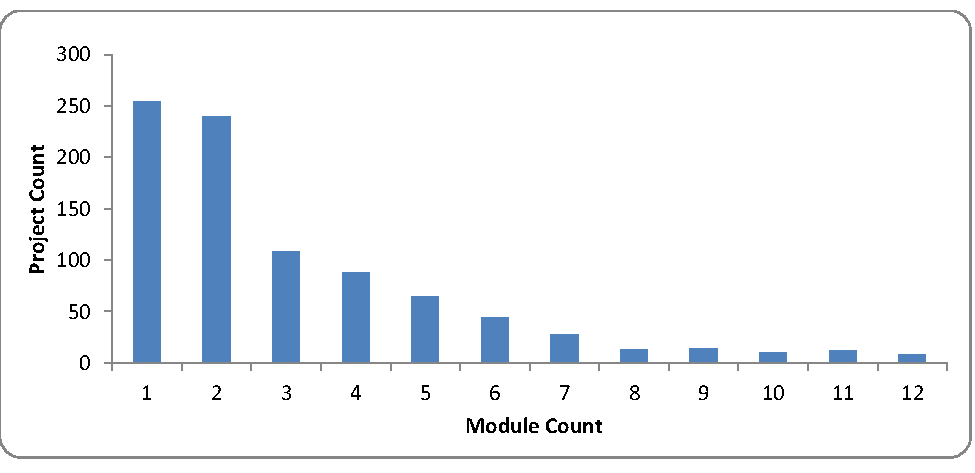
\includegraphics[width=1.0\textwidth]{ProjectModuleCount.pdf}
\caption{The number of projects grouped by the number of distinct modules within their codebase.}
\label{fig:ProjectModuleCount}
\end{figure}

\begin{figure}[htbp!] 
\centering    
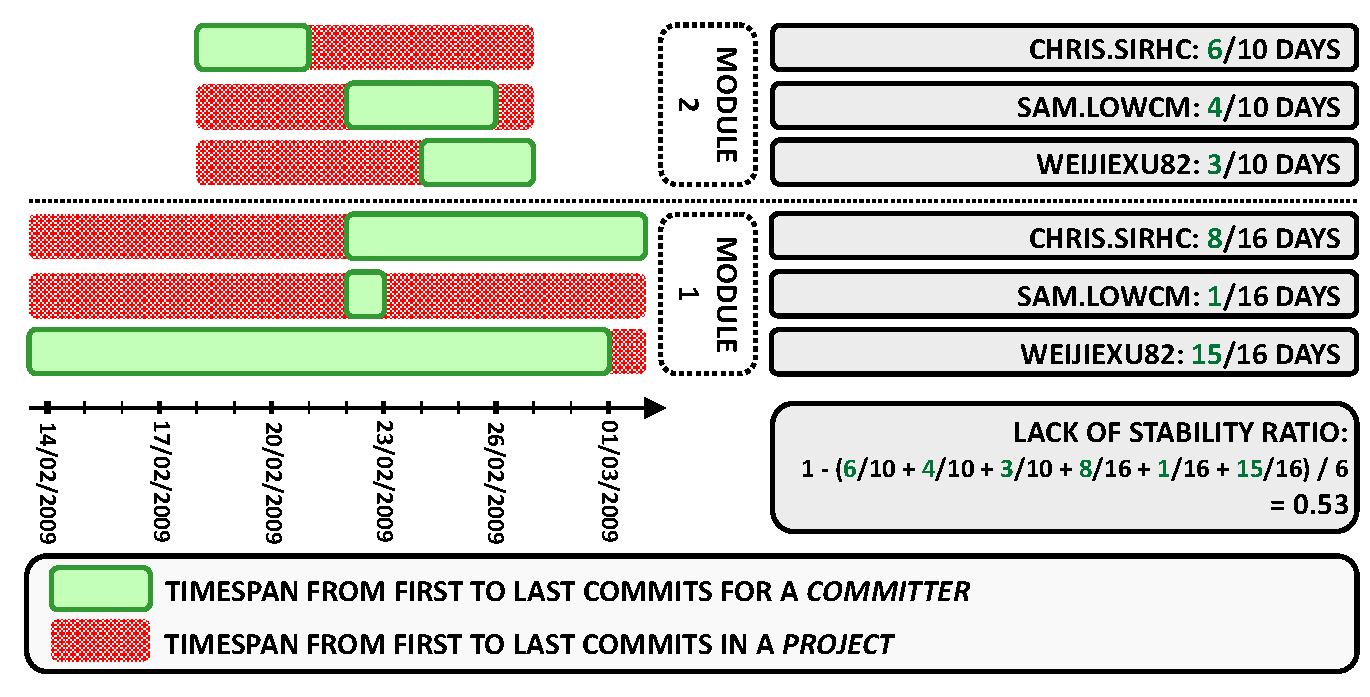
\includegraphics[width=1.0\textwidth]{IntraprojectStabilityCalcModularised.pdf}
\caption{A worked example showing the calculation of the Lack of Stability Ratio in a project called 'PipeDreamAgent' from the stability sample comprising two distinct modules.}
\label{fig:IntraprojectStabilityCalcModularised}
\end{figure}

\subsection{Validation of the Lack of Stability Ratio}
In the previous chapter, one of the key considerations was to mitigate for the fact that increasing team sizes can accompany an increase in functional complexity which could have a confounding impact. LSR is, perhaps, a less intuitive and direct measure than team size and, therefore, it is even more critical to quantify the relationship between this measure and other key factors that may have a confounding impact on CK metrics. Table ~\ref{tab:StabilityCorrelations} shows that LSR has negligible correlations to revision count, project duration and module count.

\begin{table}
\centering 
\caption{A matrix of Spearman correlation coefficients showing the relationship between various project-level variables}
\begin{tabular}
 \centering 
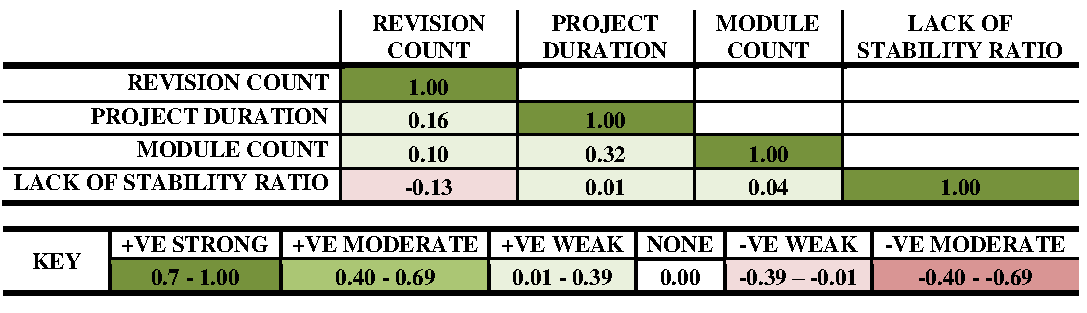
\includegraphics[width=1.0\textwidth]{StabilityCorrelationsSpearman.pdf}
\label{tab:StabilityCorrelations}
\end{tabular}
\end{table}

By way of qualitative validation, it is notable in Figure ~\ref{fig:StabilityOutliers} that the visual representation of the time-frames of activity of two outlier projects from the stability sample show features that would be expected given their respective LSR values. The project named 'Dmdirc' has a high stability ratio and it is clear that the committers to this project work together for an extended period of time with an almost total degree of overlap. Conversely, 'Cykelgarage' shows an early commit by one author followed by a lull in activity and a series of commits by five other authors with some degree of overlap. While it is arguable that this measure inordinately penalises projects with an early commit followed by a period with no committer activity, it is also worth pointing out that this is quite a rare pattern and furthermore it is helpful to capture the gap in time that elapses between periods of activity as those gaps may be associated with a loss of knowledge from the team. In this particular example the commentary in the commit logs reveal that the initial commit activity to Cykelgarage represented an substantial check-in of code representing the first set of functionalities for the software. The subsequent lull is therefore significant in that it creates distance between the initial committer and the subsequent committers to the project - an aspect that is and should be captured by LSR.

The probability distribution for LSR across the stability project sample is illustrated in Figure ~\ref{fig:StabilityDistribution} and, while visually similar to a normal distribution, the Kolmogorov-Smirnov test returns a P-value of 0.00 and a D-statistic of 0.50 revealing that half the observations reside outside a normal distribution.

\begin{figure}[htbp!] 
\centering
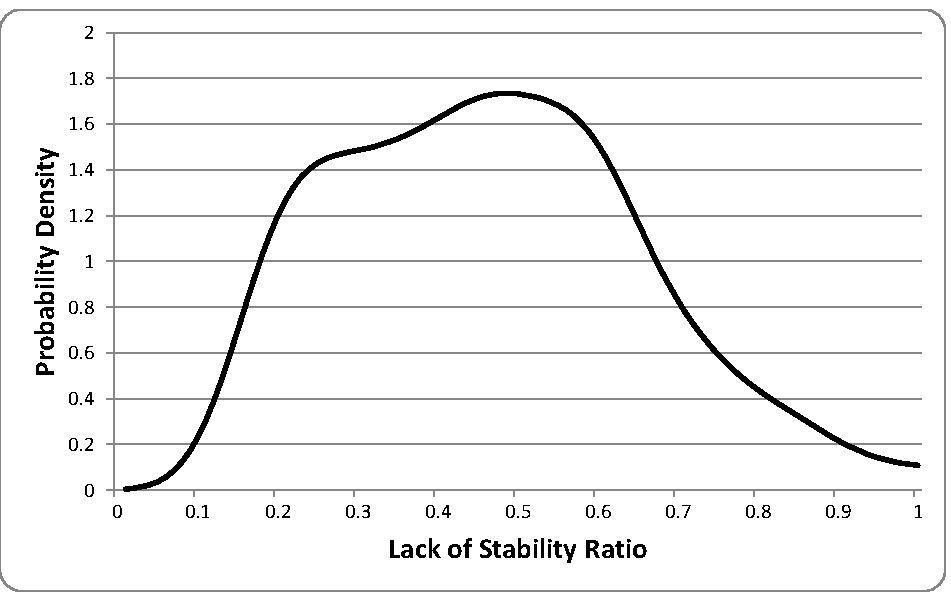
\includegraphics[width=1.0\textwidth]{StabilityDistribution.pdf}
\caption{The probability distribution for the Lack of Stability Ratio (LSR) across the stability sample.}
\label{fig:StabilityDistribution}
\end{figure}

\begin{figure}[htbp!] 
\centering    
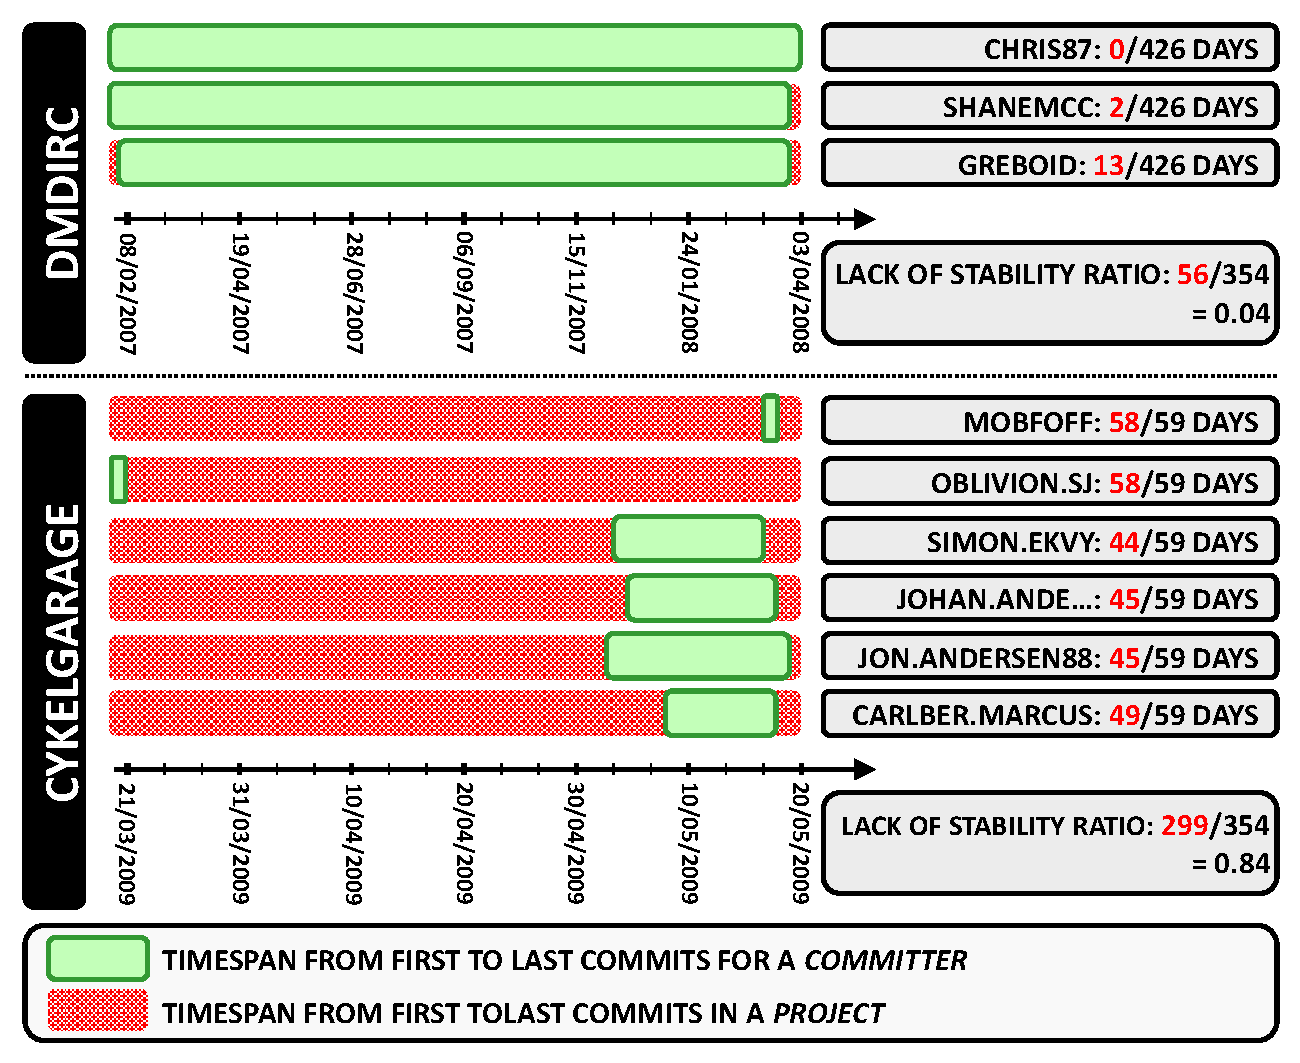
\includegraphics[width=1.0\textwidth]{StabilityOutliers.pdf}
\caption{Visualising the 'time-frames of activity' for two outlier projects: Cykelgarage and Dmdirc.}
\label{fig:StabilityOutliers}
\end{figure}

\subsection{Results}
The initial set of results visualisations are represented as scatter diagrams showing the mean CK metric values at a project level plotted against LSR for those projects. Averaging CK metrics may be misleading as it can be heavily skewed by outlier values and thus misrepresentative of the data set. That said, it can be helpful as a first step in determining if there any clear trends manifest which can then be explored further. There are two observations that can immediately be made. First, the majority of the data points exist on the left-hand-side of the plots. This is a natural given that the majority of projects exhibit LSR values lower than 0.5 as confirmed by the probability distribution depicted in ~\ref{fig:StabilityDistribution}. The second observation is that there is no clear and powerful relationship between LSR and the project averaged metric values that manifest in these plots. 

\begin{figure}[htbp!] 
\centering    
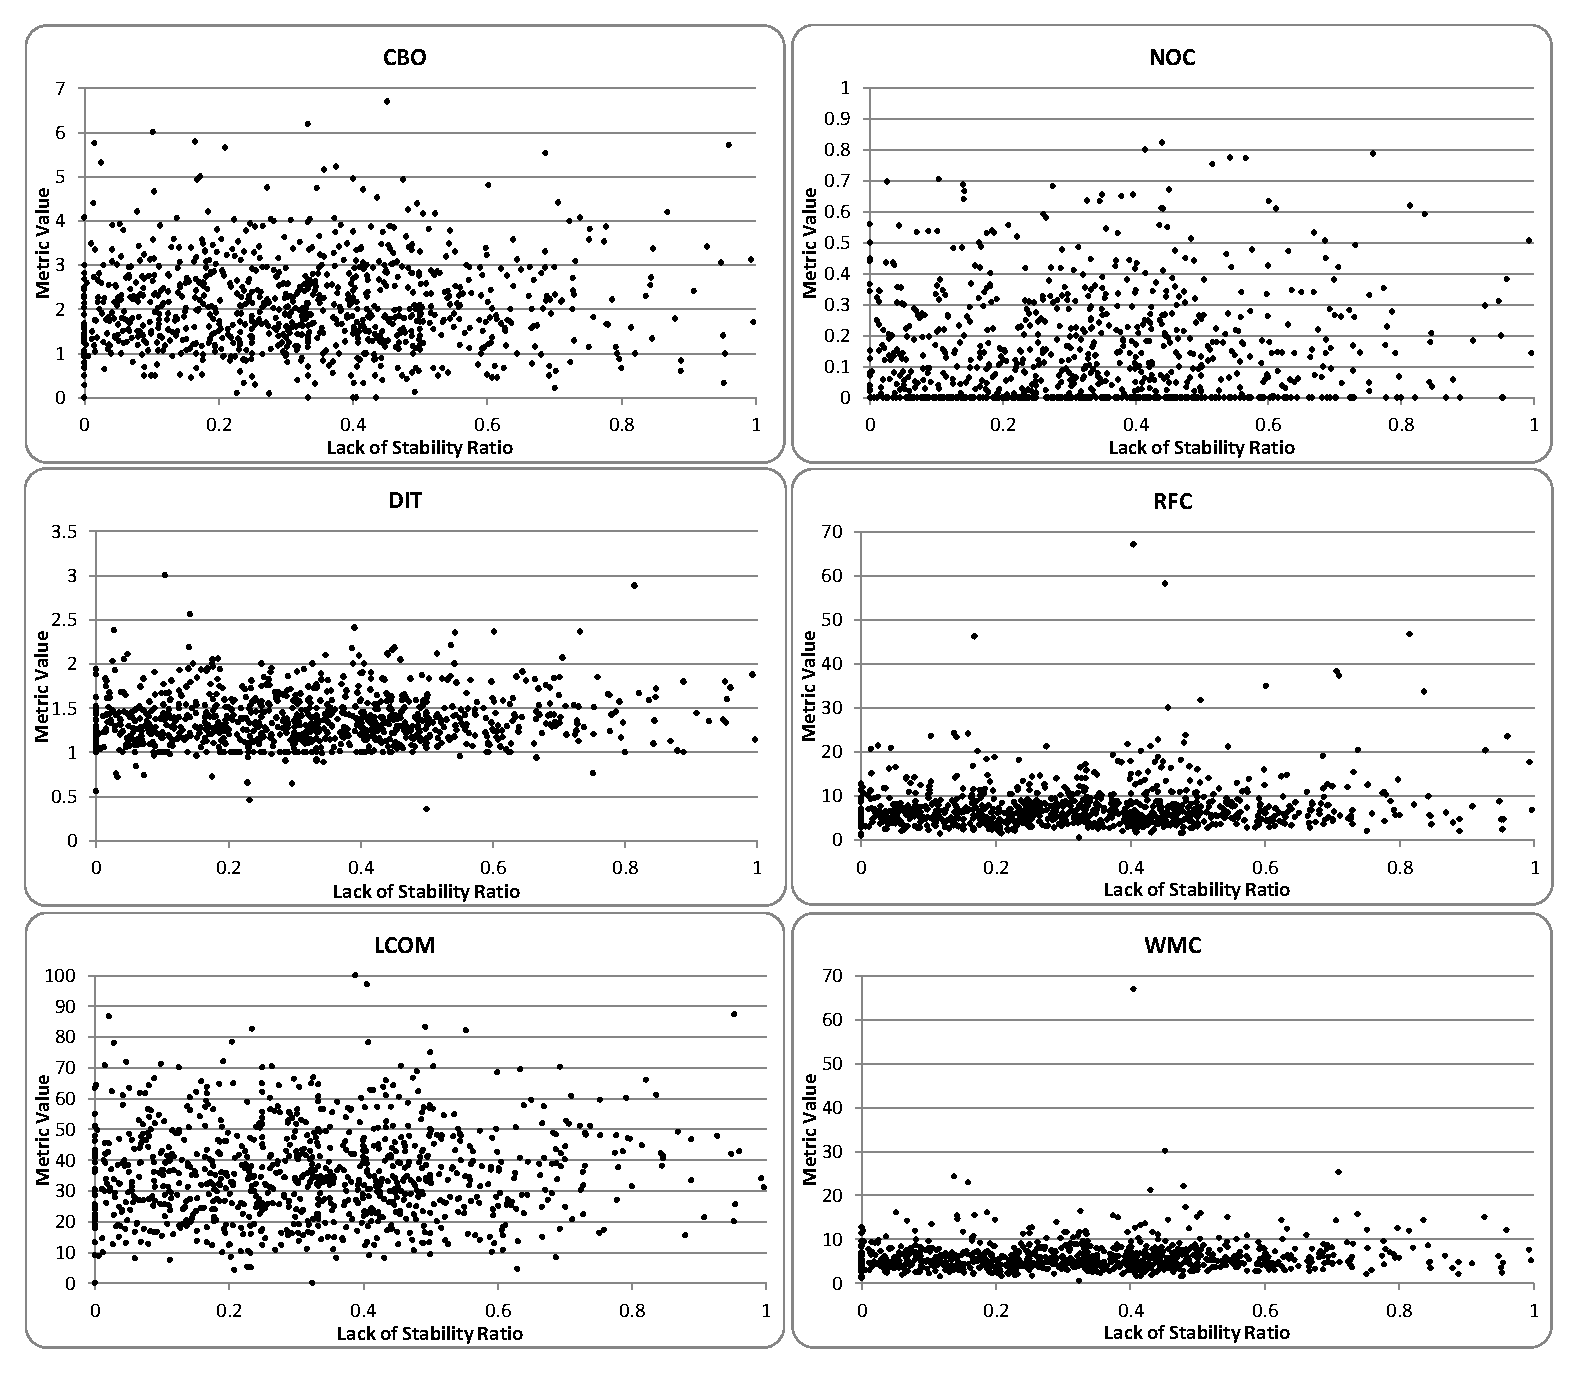
\includegraphics[width=1.0\textwidth]{ScatterDiagrams.pdf}
\caption{Scatter diagrams plotting metric values against stability ratios.}
\label{fig:ScatterDiagrams}
\end{figure}

The charts in Figure ~\ref{fig:AverageMetricStability} show mean metric values for projects exhibiting a range of stability ratios. There is a noticeable upward trend across all metric types with the exception of CBO and NOC, implying at this early stage of analysis that teams with greater stability produce projects with higher cohesion and lower inheritance complexity. 

\begin{figure}[htbp!] 
\centering    
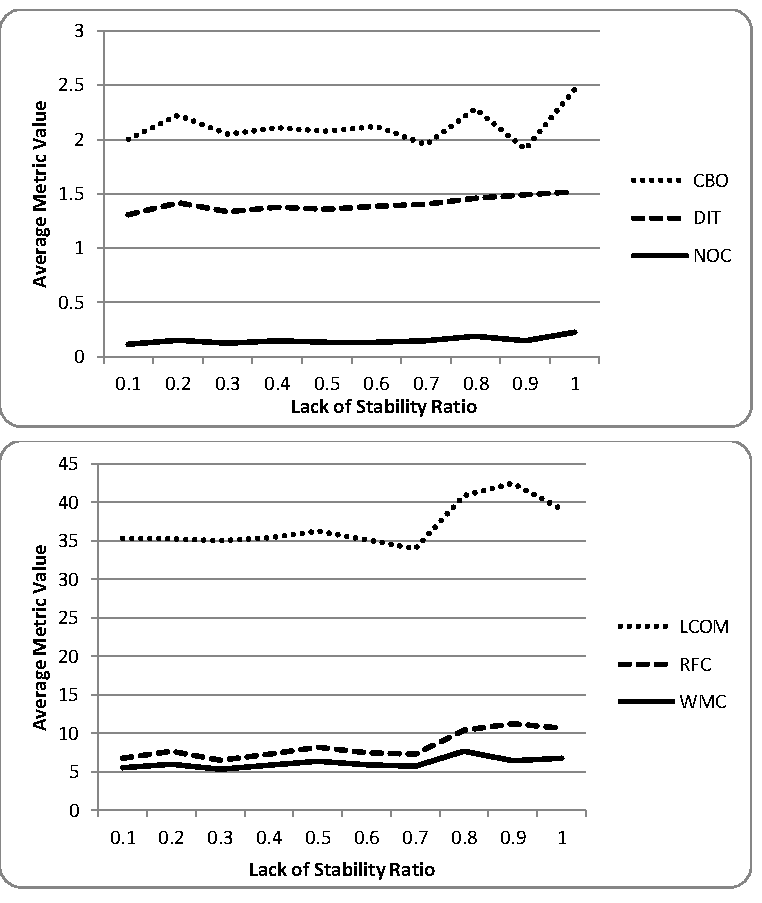
\includegraphics[width=1.0\textwidth]{AverageMetricStability.pdf}
\caption{Mean project-level metrics grouped by stability ratio (rounded up to one decimal place).}
\label{fig:AverageMetricStability}
\end{figure}

Table ~\ref{tab:BasicLinearRegressionSingleFactor} shows the results of a basic Ordinary Least Squares linear regression with LSR as the sole independent variable. In a departure from the analysis in the prior chapter, it is not necessary to include revision count into this model as the correlation analysis in Table ~\ref{tab:StabilityCorrelations} shows that LSR does not track any of the key project-level factors and therefore those factors should not have a confounding impact. The model can be expressed as follows where LSR is multiplied by a coefficient ($\beta$), $\gamma$ is the intercept, and  $\epsilon$ is the standard error:

\[\large Metric \: Value = \beta_{LSR}\, LSR +  \gamma + \epsilon \]

A number of observations can be made based on the results in Table ~\ref{tab:BasicLinearRegressionSingleFactor}.

\begin{itemize}
\item  \textbf{Rejection of null hypothesis H0,2:} The R-Squared values show that LSR can explain a high proportion of the variance observed in the DIT and LCOM metrics, a substantial proportion of the variance of CBO, and a minimal element of the variance of RFC and WMC. All regressions report a p-value < 0.005 - i.e. the Bonferroni corrected $\alpha$ - and can be considered highly significant. CBO captures coupling and modularity, DIT captures inheritance complexity and LCOM captures coupling. Consequently, this model provides support for the alternative hypothesis H1,2.1 that \textit{'less stable development teams produce software exhibiting higher coupling, higher complexity, lower cohesion and lower modularity'}.

\item  \textbf{Stability has a powerful impact on CBO, DIT and LCOM:} The high coefficient estimates show that LSR has a fairly powerful impact on the CBO, DIT and LCOM metrics. For instance, the 8.67 coefficient reported in the CBO column indicates that a movement of 0.1 in LSR would have a 0.87 impact on the CBO: a metric with a mean of 3.55 within the stability sample. The low standard errors and high T-statistics show that this linear model provides a reasonable fit.
\end{itemize}

\begin{table}
\centering 
\captionof{table}{Results of the OLS linear regression with intra-project stability as a single independent variable.}
\begin{tabular}
 \centering 
 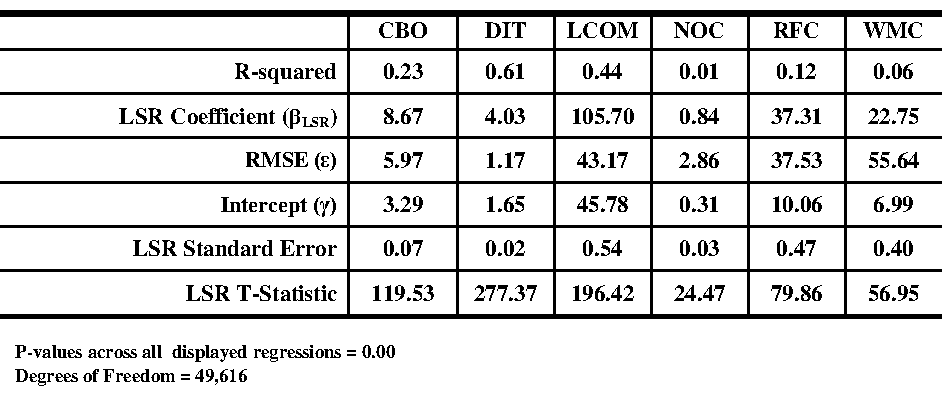
\includegraphics[width=1.0\textwidth]{BasicLinearRegressionSingleFactor.pdf}
 \label{tab:BasicLinearRegressionSingleFactor}
\end{tabular}
\end{table}

While this result evidences the impact of LSR on CK metrics, the 'idiosyncratic' project features referred to in Chapter 4 (previously established to play a significant role in the relationship between team size and CK metrics) is likely to play a role in determining how LSR impacts the structural attributes of individual projects. To take a hypothetical but intuitive example, if a software development team is geographically collocated and working on a highly complex problem, stability should have greater predictive power than for a development team that is geographically dispersed and working on a relatively simple problem solving to established and documented design patterns. While individually establishing the impact of these myriad of factors is well beyond the scope of this work, using the 'Linear Mixed Models' (LMM) statistical approach can, as demonstrated in Chapter 4, provide a linear regression which factors in this idiosyncratic component to establish coefficients with greater accuracy, reducing residual errors in the process. This can be expressed in a similar way to the equation in the previous section where $\gamma_p$ is now the project-specific intercept:

\[\large Metric \: Value = \beta_{LSR}\, LSR +  \gamma_p + \epsilon \]

Table ~\ref{tab:RandomInterceptsLinearRegressionSingleFactor} shows the results of the LMM regression and the following observations can be made. 

\begin{itemize}
\item  \textbf{Sample variance is substantially higher than group variance:} As observed with the LMM models of the previous chapter, the groups exhibit lower variance than the overall sample confirming the significant influence that the  project-specific idiosyncratic characteristics have on CK metric values.
\item  \textbf{Lower Residuals:} Again, consistent with the application of LMMs in the previous chapter, Table ~\ref{tab:RandomInterceptsLinearRegressionSingleFactor} shows substantially lower residuals across all metric regressions when compared to the OLS results in Table ~\ref{tab:BasicLinearRegressionSingleFactor}. 
\item  \textbf{Lower coefficient estimates:} The lower coefficient estimates in the LMMs indicate that team stability has less impact on metric values than otherwise apparent in the OLS regression. This is only noteworthy in the context of highlighting that LMMs revise the coefficient estimates to reduce residuals given the flexibility of project-specific intercepts.

\end{itemize}

\begin{table}
\centering 
\captionof{table}{Results of the 'random intercepts' linear regression with intra-project stability as a single categorical independent variable with observations grouped by project.}
\begin{tabular}
 \centering 
 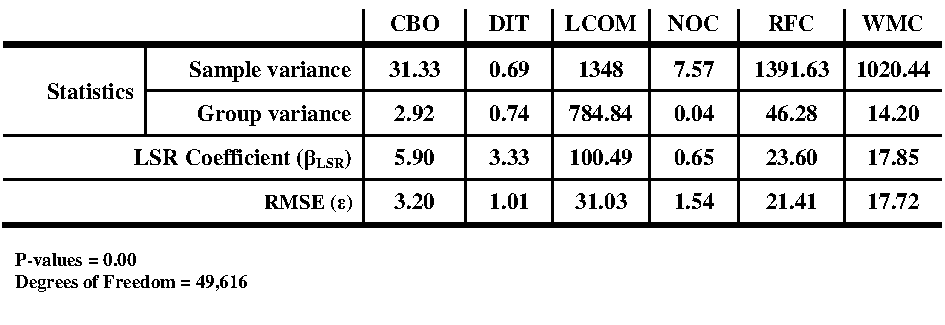
\includegraphics[width=1.0\textwidth]{RandomInterceptsLinearRegressionSingleFactor.pdf}
 \label{tab:RandomInterceptsLinearRegressionSingleFactor}
\end{tabular}
\end{table}

\section{Inter-project stability analysis} %Section - 5.5
While studying intra-project stability enables the quantitative analysis of the impact of stability on the structural metrics of software, it is also informative to study at another key dimension of team stability: namely the impact of \textit{inter-project stability} on structural metrics; that is the stability that is gained through a development team retaining a consistent set of committers across multiple projects. This variant of stability intuitively can bear relevance to those practitioners looking to understand how continuing with an unchanged development team can bring benefits to internal and external attributes of the produced software. For this analysis the same null and alternate hypothesis hold as in the previous section: H0,2 and H1,2.1 respectively.

\subsection{Analysis approach}
As documented earlier in Section 5.4 of this chapter, there are a number of criteria that are applied in order to obtain a dataset that lends itself well to contrasting by inter-project team stability: namely that the project timelines should not overlap and that the chronologically later project should not contain any committers that did not exist in the earlier project. The nature of the subsequent analysis is twofold. First, the metrics of projects within 'stable project pairs' are compared to each other as depicted in Figure \ref{fig:StabilityAnalysis}. The second analysis is a linear regression to model the relationship between inter-project team stability and CK metrics.

To perform a linear regression, it is necessary to derive a categorical measure of lack of stability which can serve as an independent variable acting on CK metrics as dependent variables within the linear model. To achieve this the model assigns a binary with a value of '1' assigned to the first (chronologically) of a stable project pair and '0' assigned to the second project in the pair. This is an approach that attributes a total lack of team stability to the earlier project and total stability to the later project of the stable project pair. This is a simplification as it is entirely conceivable that any project team may have collaborated previously on other projects outside the GoogleCode forge and thus not captured within our data set and not reflected in this measure of lack of stability. Furthermore, in this analysis no account is made of the intra-project stability that accrues through the course of the earlier or the later project within a pair. These simplifications do not constitute a significant threat to the validity of this analysis as there is certainly an accumulation of inter-project stability from the earlier project to the later project within the stable project pair, enabling meaningful observations to be made. However, this measure leaves some scope for refinement as will be discussed in the Future Work in the next chapter of this thesis.

\begin{figure}[htbp!] 
\centering    
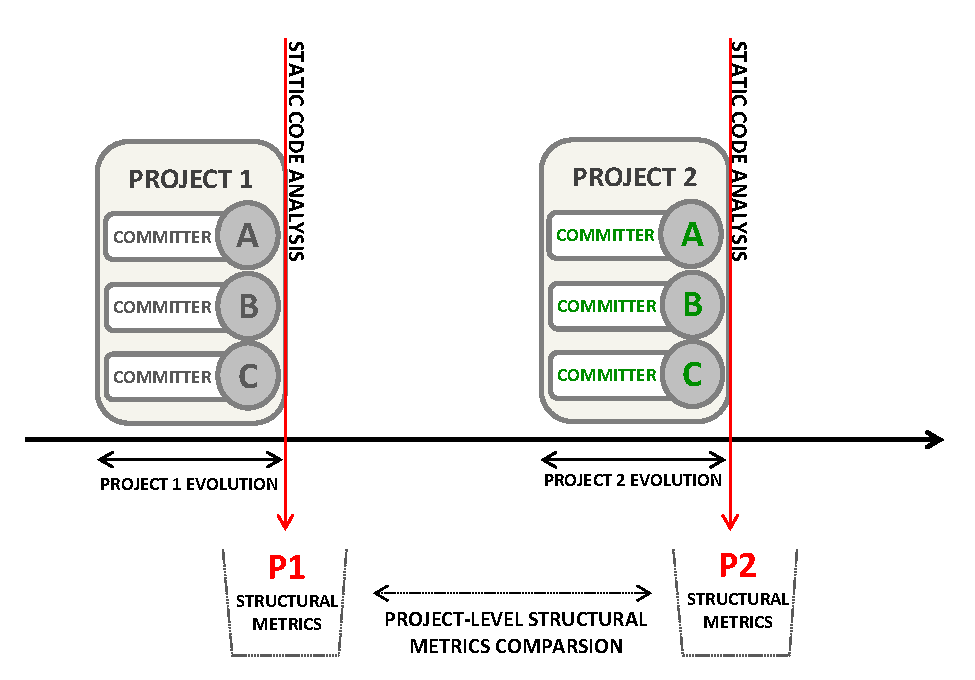
\includegraphics[width=1.0\textwidth]{StabilityAnalysis.pdf}
\caption{An illustration of the inter-project stability analysis approach.}
\label{fig:StabilityAnalysis}
\end{figure}

\subsection{Results}
Figure ~\ref{fig:InterprojectSignificance} shows the result of the first phase of analysis detailing the proportion of 'stable project pairs' where the structural metrics of the each member of the pair exhibit a significant difference from the other with a 95\% confidence interval; i.e. a Mann-Whitney test returning p-values of < 0.05. Significant difference across a large proportion of projects are observed - from a maximum of 38\% for RFC to a minimum of 22\% for NOC. Consistent with the inter-project stability analysis, this is further rejection of null hypothesis H0,2 that \textit{'Development team stability does not impact the coupling, complexity, cohesion or modularity of the produced software'}. The nature of this difference is studied, as in the prior analyses in this thesis, through linear modelling.

\begin{figure}[htbp!] 
\centering    
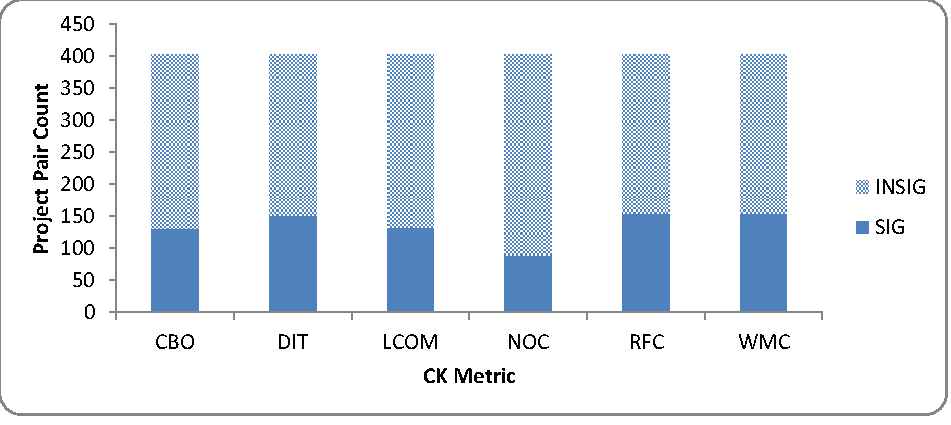
\includegraphics[width=1.0\textwidth]{InterprojectSignificance.pdf}
\caption{A chart showing the number of project pairs that show a significant difference (i.e. p-values < 0.05) between the metrics of each project in the pair. }
\label{fig:InterprojectSignificance}
\end{figure}

Table ~\ref{tab:BasicLinearRegressionInterprojectStability} details the results of an OLS linear regression with the categorical binary lack of stability measure as a single independent variable. Table ~\ref{tab:RandomInterceptsLinearRegressionInterproject} shows the results of the LMM Regression. The following observations can be made from these results.


\begin{itemize}
\item  \textbf{Further rejection of null hypothesis H0,2:} The R-squared values show that a substantial proportion of the DIT and LCOM metrics variance is explained by this inter-project lack of stability. The positive coefficients along with the low standard errors relative to those coefficients shows that CK metrics trend positively with inter-project lack of stability; a result consistent with the observations in the earlier intra-project stability analysis. This result provides further support for alternative hypothesis H1,2.1 that �less stable development teams produce software exhibiting higher coupling, higher complexity, lower cohesion and lower modularity�.

\item  \textbf{LMM results consistent with previous results:} When compared to the basic OLS regression, as with the intra-project analysis, the coefficient estimates are lower (with broadly lower residuals) given the project-specific intercepts of the LMM regression.
\end{itemize}

\begin{table}
\centering 
\captionof{table}{Results of the 'ordinary least squares' linear regression with inter-project stability as a single categorical independent variable.}
\begin{tabular}
 \centering 
 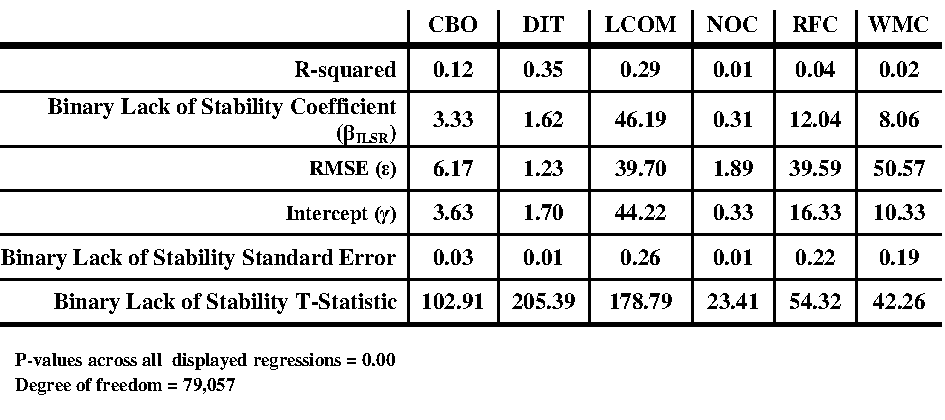
\includegraphics[width=1.0\textwidth]{BasicLinearRegressionInterprojectStability.pdf}
 \label{tab:BasicLinearRegressionInterprojectStability}
\end{tabular}
\end{table}

\begin{table}
\centering 
\captionof{table}{Results of the 'random intercepts' linear regression with inter-project stability as a single categorical independent variable with observations grouped by project.}
\begin{tabular}
 \centering 
 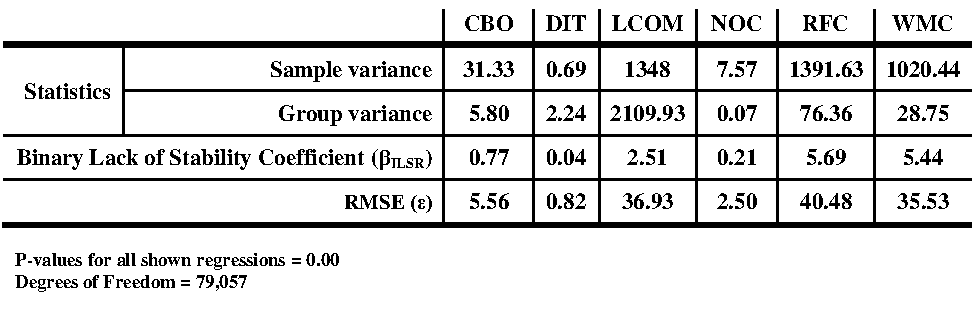
\includegraphics[width=1.0\textwidth]{RandomInterceptsLinearRegressionInterproject.pdf}
 \label{tab:RandomInterceptsLinearRegressionInterproject}
\end{tabular}
\end{table}


\section{Results at a Project Level} %Section - 5.7
\subsection{Project Selection}
Applying PCA to the team stability sample, a new set of loading coefficients emerge as documented in Table ~\ref{tab:TeamStabilityPCA}. It is notable that LSR hardly features in the first principal component. This can be explained by the fact that LSR explains a great deal of variance in the CK metrics - variance which is captured through the substantial loading coefficients on the CK metrics themselves. Figure ~\ref{fig:TeamStabilityScatter} shows the sample scattered by the two principal components.

\begin{table}
\captionof{table}{Loading coefficients of the Principal Component Analysis as applied to the team stability analysis sample.}
\begin{tabular}
 \centering 
 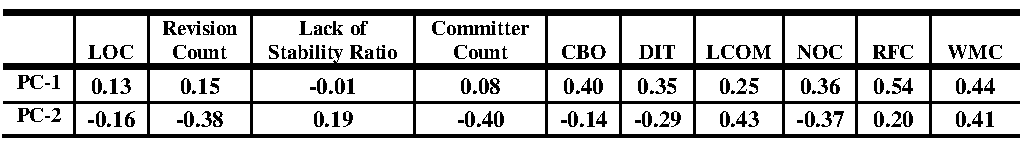
\includegraphics[width=1.0\textwidth]{TeamStabilityPCA.pdf}
 \label{tab:TeamStabilityPCA}
\end{tabular}
\end{table}

\begin{figure}[htbp!] 
\centering    
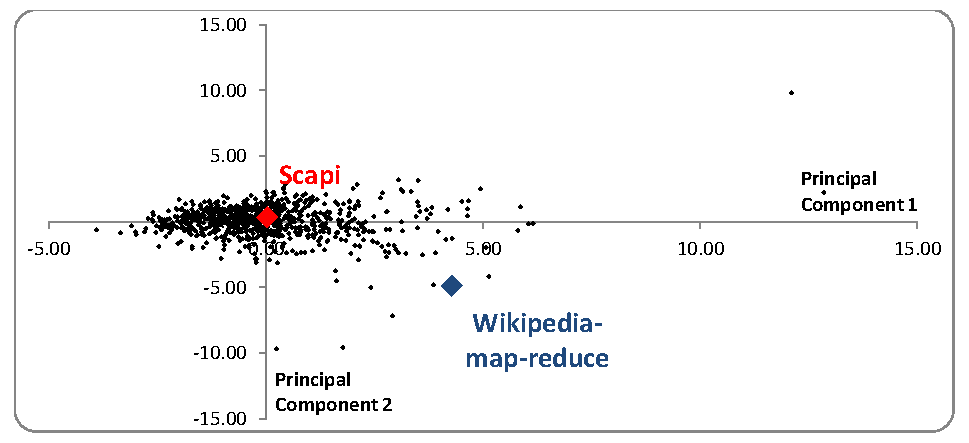
\includegraphics[width=1.0\textwidth]{TeamStabilityScatter.pdf}
\caption{A visualisation of the team size sample scattered across the two principal components. The selection of Aviator and Precise for further study.}
\label{fig:TeamStabilityScatter}
\end{figure}

Through the intra-team stability analysis, the broad trends observed were that DIT, LCOM, RFC, WMC trended positively with LSR. Two projects were selected with varying LSR values exhibiting relative metrics trends similar to those broader trends. Wikipedia-map-reduce and Scapi have LSR values of 0.41 and 0.15 respectively indicating that the latter has a project team which is substantially more stable. These particular projects were chosen as have similar revision counts (129 and 157 respectively) and five unique committers each. The two projects appear in distant positions from one another in Figure  ~\ref{fig:TeamStabilityScatter} with Scapi residing close to the centre of the cluster while Wikipedia-map-reduce is very much an outlier owing to its high RFC and WMC values.

Wikipedia-map-reduce is an API that allows analysis of Wikipedia using the Hadoop Map-Reduce framework for parallel processing. Is is purely server-side software with no graphical interface. Scapi is a loan administration system which forms the basis of a company called Montep�o Plus which operates as an online pawn shop, swapping various personal items or assets for cash. 

Although both projects share the same team size, a deeper analysis of committer behaviour analysis depicted in Figure  ~\ref{fig:ScapiWikipediaMapReduceCommitterAnalysis} shows that Wikipedia-map-reduce has a single prolific contributor who is responsible for the majority of the codebase while Scapi's five committers more equitably distributed responsibility of the codebase amongst themselves. In the next chapter more consideration will be given to the role of 'core' committers versus that of 'peripheral' committers and how this can present both a threat to validity and an opportunity for further work.

\begin{figure}[htbp!] 
\centering    
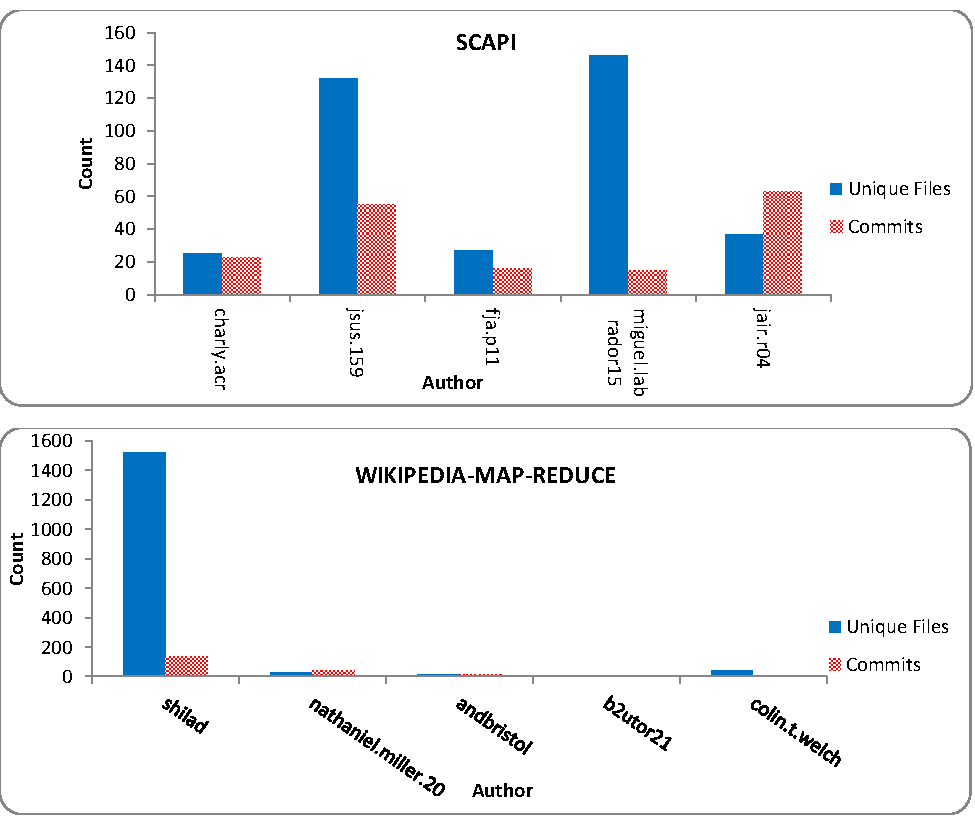
\includegraphics[width=1.0\textwidth]{ScapiWikipediaMapReduceCommitterAnalysis.pdf}
\caption{Committer behaviour analysis for the Scapi and the Wikipedia-Map-Reduce projects.}
\label{fig:ScapiWikipediaMapReduceCommitterAnalysis}
\end{figure}

\begin{figure}[htbp!] 
\centering    
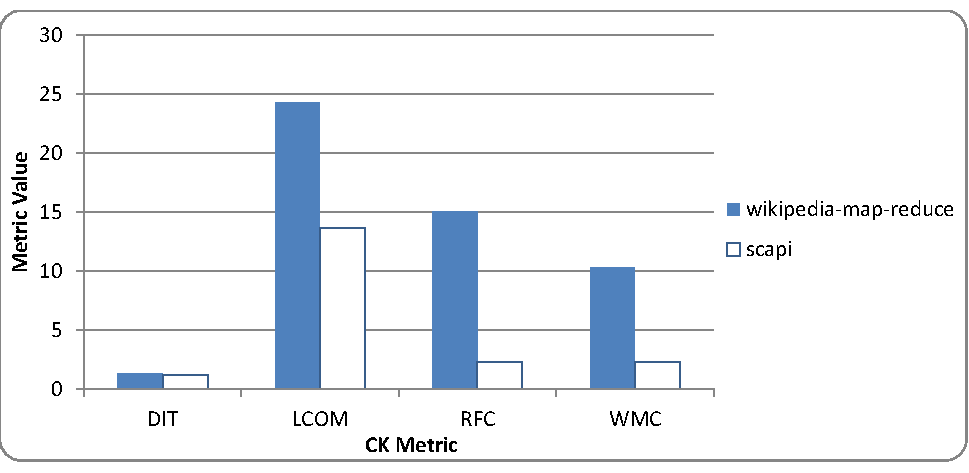
\includegraphics[width=1.0\textwidth]{TeamStabilityResultsCompare.pdf}
\caption{Key structural attributes for Wikipedia-map-reduce compared against Scapi.}
\label{fig:TeamStabilityResultsCompare}
\end{figure}

\subsection{Project Comparison}
Through qualitatively reviewing the code in both Scapi and Wikipedia-map-reduce, the latter emerges as the more structurally complex of the two projects. Although there is certainly less to critique in Wikipedia-map-reduce than in the previously reviewed Precise project - an observation which is consistent with the lower absolute LCOM and RFC numbers in Wikipedia-map-reduce relative to Precise - there are still some examples of poor encapsulation and inordinate structural complexity which will lead to poor cohesion, high coupling and low modularity. The Encoder class is an example of this as the code snippet in Figure ~\ref{fig:StabilityExample} highlights. It is an excessively large class at 1616 lines, 34 methods and four distinct inner classes. This class is fairly anomalous within the broader codebase which is generally well written.

In Wikipeda-map-reduce there is substantially more use of inheritance which confirms the higher DIT compared to Scapi (1.36 and 1.16 respectively). This is largely driven by the fact that Wikipedia-map-reduce has a substantial library of collections implementations which functionally lend themselves well to sharing behaviour via inheritance. 

Table  ~\ref{tab:RandomInterceptsSelectedProjects} documents the intercept and residual values for the Scapi and Wikipedia-map-reduce projects from the intra-project LMM regression. As was observed the similar analysis of team size in Chapter 4, the project that is more distant from the centre of the cluster exhibits higher residuals - in this case Wikipedia-map-reduce. This is attributable to the fact that the coefficient estimates of the regression line will be dominated by those non-outlier projects that make up the main cluster in the scatter plot and consequently show lower residuals. The intercept values are more difficult to interpret and are influenced by two key factors. The first is that Wikipedia-map-reduce has higher metric values which will influence a higher intercept value. However, given that the LSR is higher for this project, the regression line will have �further to travel� along the x-axis in order to intercept with the y-axis, which causes a decrease in the intercept values. As a result, the intercepts are a mixed bag with Wikipedia-map-reduce showing higher intercept values for CBO, DIT, NOC and RFC and lower intercept values for LCOM and WMC. 

\begin{table}
\centering 
\captionof{table}{The intercepts and residuals for the Scapi and Wikipedia-ma-reduce projects.}
\begin{tabular}
 \centering 
 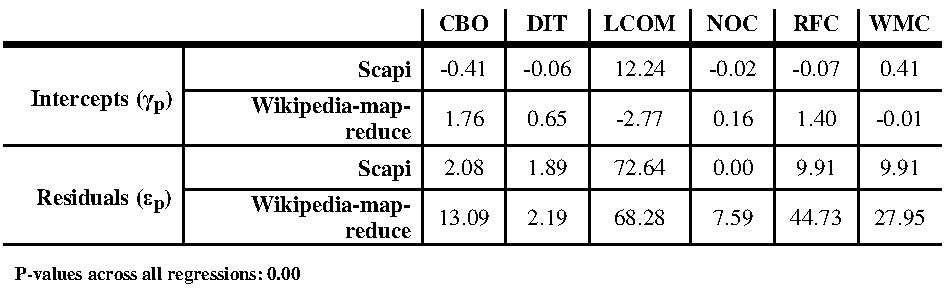
\includegraphics[width=1.0\textwidth]{RandomInterceptsSelectedProjects.pdf}
 \label{tab:RandomInterceptsSelectedProjects}
\end{tabular}
\end{table}

While the team stability analysis has accurately identified project teams with a higher lack of stability  produces software with degraded structural attributes (from a maintainability standpoint), there are other influencing factors given that stability cannot explain all the variance in the structural metrics of the software. Of these project-specific 'idiosyncratic factors', such as relative experience levels or problem domain knowledge, further analysis would be beneficial but is beyond the scope of this work.

\begin{figure}[htbp!] 
\centering    
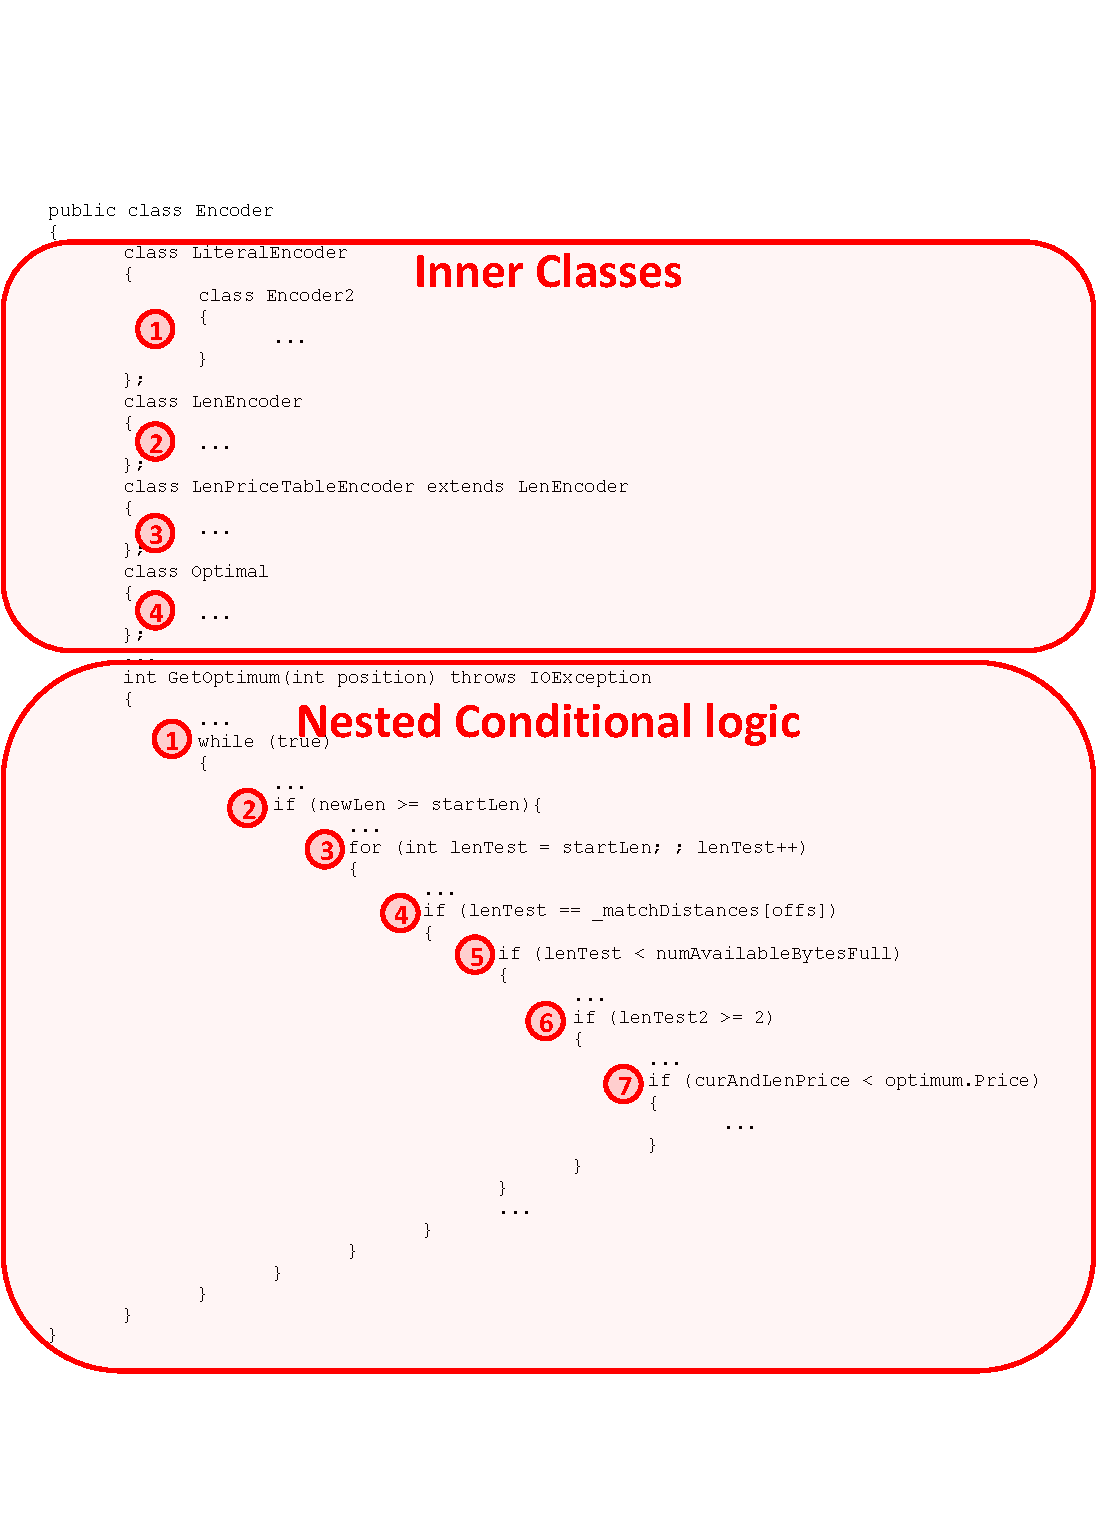
\includegraphics[width=1.0\textwidth]{StabilityExample.pdf}
\caption{A code snippet from Encoder class within the Wikipedia-map-reduce project. Multiple inner classes and nested iterative blocks are numerically labelled.}
\label{fig:StabilityExample}
\end{figure}

\section{Summary} %Section - 5.8
A number of observations can be made as a result of the analyses in this chapter. The intra-project stability analysis yielded clear trends with the introduction of the LSR measure being central to the analysis. Those teams exhibiting greater stability exhibited structural metrics that tended to be lower across measures of structural complexity and cohesion. The trends on inter-project stability were similar. The approach of mining for 'stable project pairs' proved to be a useful approach in contrasting metric populations, showing significant difference between the structural metrics of the project pairs across a large proportion of the stability analysis data set. The linear regressions proved that a substantial portion of the variance with the sample was attributable to the categorical measure of lack of stability. However, the R-squared values were lower in comparison to the intra-project stability linear model, possibly attributable to the lower precision associated with the inter-project binary categorical lack of stability measure.

Given the negative correlation between these structural metrics and fault-proneness, it can be confirmed that the observations within this chapter are consistent with the work of Huckman et al. \citep{huckman2009team} and Gardner et al. \citep{gardner2012dynamically} who found that greater team stability was associated with lower fault-proneness. Referring, again, to table 2.4 (the survey of research correlating CK metrics to the sub-attributes of maintainability), inferences can be drawn from the observed structural trends against the impact on the maintainability of the software. With the results in this chapter showing that lack of cohesion, coupling and inheritance complexity tend to increase against a decreasing team stability, and given the already established negative correlations between the impacted CK metrics and maintainability in the prior literature, it can be deduced that lower team stability leads to lower software maintainability. This is depicted in Figure ~\ref{fig:ResultOverview} and allows for a rejection of null hypothesis  H0,2 and a confirmation of the alternative hypotheses H1,2.1 and H1,2.2.

\begin{figure}[htbp!] 
\centering    
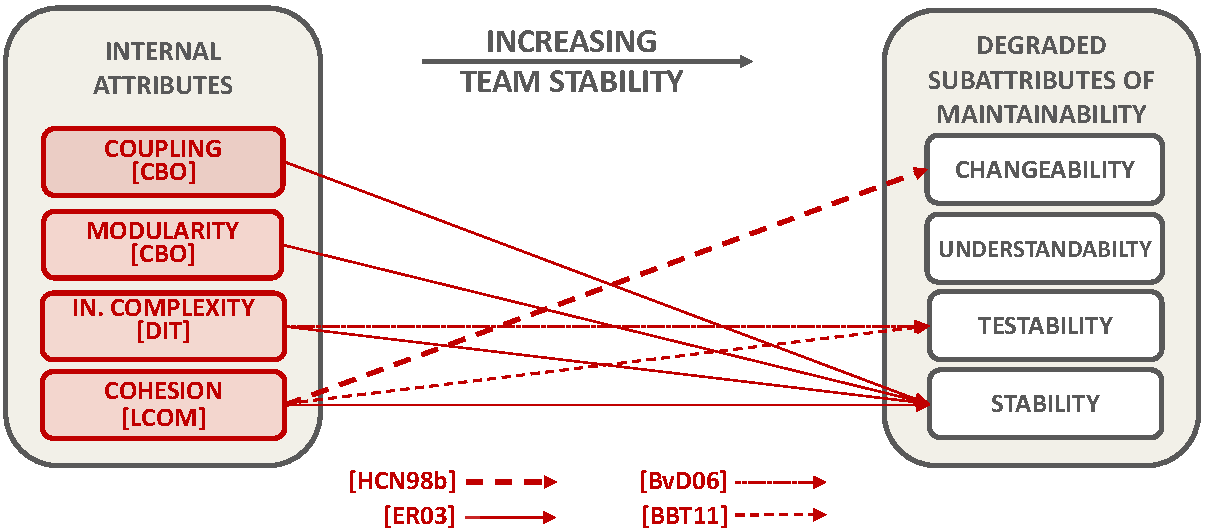
\includegraphics[width=1.0\textwidth]{ResultOverview.pdf}
\caption[Summary of the results of the Intra-project stability analysis.]{Summary of the results of the Intra-project stability analysis. This analysis shows similar trends to the team size analysis with Changability, Testability and Stability all associated with a degradation inline with the observed trends within the structural metrics.}
\label{fig:ResultOverview}
\end{figure} 
 
\section{Chapter Review} %Section - 5.9
This chapter studied the relationship between team stability and the CK metrics of the produced software. As in the previous chapter, at the outset the sample extraction and exploratory data analysis was presented. The two measures of Inter-project and intra-project team stability were defined and modelled individually. The linear models were developed and analysed in conjunction with specific projects from within the sample. 

The next chapter is a discussion primarily covering the contribution to knowledge within this thesis, threats to validity, and potential avenues of future work.